\documentclass[11pt]{book}

% Essential
\usepackage[dutch]{babel}
\usepackage{titling}
\usepackage{tikz}
\usetikzlibrary{decorations.text,calc,arrows.meta}
%\usetikzlibrary{scopes,chains,shapes,positioning}
\usetikzlibrary{mindmap}
\usepackage{pdfpages}
% Optional
\usepackage{microtype}
\usepackage{hyperref}
\usepackage{amsmath,amsthm,amsfonts,amssymb}
\usepackage{graphicx}

% Titleplage
\newcommand{\theauthors}{Seppe Duw\'e}
\newcommand{\thecontributors}{Xavier Dejager}
\newcommand{\theprofs}{S. Vandewalle, M. Van Barel}

\title{Numerieke modellering en benadering \\ (B-KUL-H01P4a)}
\date{\today}
\author{\theauthors}

% Margins
\setlength{\topmargin}{0in}
\setlength{\footskip}{0.5in}
\setlength{\textwidth}{6.5in}
\setlength{\oddsidemargin}{0in}
\setlength{\evensidemargin}{0in}
\setlength{\textheight}{8.5in}

% Image folder
\graphicspath{{figures/}{../figures/}}

% Theorem styles
% declare a new theorem style
\newtheoremstyle{mystyle}%
{}% Space above
{}% Space below 
{\itshape\color{blue}}% Body font
{}% Indent amount
{}% Theorem head font
{.}% Punctuation after theorem head
{ }% Space after theorem head 
{}% Theorem head spec (can be left empty, meaning ‘normal’)

\theoremstyle{mystyle}
\newtheorem{defn}{Definitie}[section]
\newtheorem{exam}{Examen}[section]
\newtheorem{exmp}{Voorbeeld}[section]
\newtheorem{form}{Formularium}[section]
\newtheorem{tip}{Tip}[section]
\begin{document}
\frontmatter
% Title Page
\begin{titlepage}

\thispagestyle{empty}

\begin{minipage}{\textwidth}
	\includegraphics[width=60mm]{logokuleng.pdf}
\end{minipage}

\vspace{40mm}

\begin{minipage}{\textwidth}
	\Huge
	\sffamily
	\thetitle
\end{minipage}

\vspace{50mm}

\hfill
\begin{minipage}[t]{0.5\textwidth}
	\Large
	\sffamily
	\textbf{Professoren} \\
	\theprofs
\end{minipage}%
\begin{minipage}[t]{0.5\textwidth}
\begin{flushright}
	\Large
	\sffamily
	\textbf{Auteurs} \\
	\theauthor
	\vspace{10mm} \\
	\textbf{Bijdragers} \\
	\thecontributors
\end{flushright}
\end{minipage}
\vfill
\end{titlepage}
% Table of Contents Page
\tableofcontents
\chapter*{Voorwoord}
Dit document bevat een beknopte samenvatting van het boek en de notities van de jaren 2016-2018. Voor de Harry Potter fans, ooit als eens in het boek van de half-bloed prins willen lezen..., of voor de 'Wat als' fans $\rightarrow$ \url{https://www.youtube.com/watch?v=eizOd7_d9pA}. Dit document bevat handige info voor het examen.  De cursus wordt gedoceerd door 2 docenten, Prof. Van Barel Marc \& Prof. Vandewalle Stefan. En bestaat uit 16 lessen, 8 oefenzittingen en 2 opgaves (Matlab of Python), eerste 8 lessen worden gegeven door Prof. Vandewalle, de laatste 8 lessen door Prof. Van Barel. 

De broncode en de laatste versie van dit document bevinden zich op \url{https://github.com/seppeduwe/NMEB}. We moedigen toekomstige lezers aan bij te dragen aan de ontwikkeling van dit document.

\section*{De proffen}
Beiden behoren ze tot NUMA (Numerieke analyse en toegepaste wiskunde) afdeling van het departement computerwetenschappen, Prof. Vandewalle houdt zich bezig met ontwikkelen van rekentechnieken in het domein van numerieke wiskunde. Prof. Vandewalle zijn expertise is vooral in numerieke methodes voor het oplossen van differentiaal vergelijken alsook in de wiskunde van computergesteund design. Prof. Van Barel gespecialiseerd in de numerieke wiskunde en dan vooral in de numerieke lineaire algebra, oplossen van stelsel, eigen waarde problemen, kleinste kwadraten problemen.
Voor het deel van Prof. Vandewalle is er een cursus beschikbaar in de Acco, geen slides en notities op het bord. Voor het deel van Prof. Van Barel zijn slides beschikbaar op Toledo en wordt het boek "Numerical Linear Algebra - Lloyd N. Trefethen David Bau" aangeraden.

\section*{Evaluatie}
Klassiek examen, 2 docenten tegelijk aanwezig, 1 examen voor de 2 delen. 4 tal vragen (bestaande uit 1 bewijs en overzichtsvragen), schriftelijke voorbereiding, bij beiden docenten langsgaan. Practica's tellen voor 4/20 punten mee. Moet voor het praktisch en theoretisch gedeelte slagen.

\section*{Syllabus}
De syllabus bevindt zich op \url{https://onderwijsaanbod.kuleuven.be/syllabi/n/H01P3AN.htm}

\section*{Doelstellingen}
Deze cursus behandelt een aantal belangrijke numerieke methoden en algoritmen die toepassing vinden in verschillende ingenieursdisciplines. De student krijgt een overzicht in de numerieke eigenschappen van deze algoritmen, hun complexiteit, nauwkeurigheid en betrouwbaarheid.
De student leert zo het kritisch evalueren van algoritmen zodat hij een gefundeerd oordeel kan vormen over voor- en nadelen van alternatieve algoritmen. De cursus besteedt ook aandacht aan het gebruik van deze algoritmen in toepassingen. De student leert hierdoor numerieke resultaten correct te interpreteren.
De student verwerft hierdoor de nodige kritische wetenschappelijke houding binnen dit onderzoeksdomein. In de practica en in de oefenzittingen gebruikt de student de programmeeromgeving Matlab. De resultaten die de student bekomen heeft in de practica worden via een verslag gerapporteerd. Dit is  een oefening in schriftelijk rapporteren. Door in de hoorcolleges en oefenzittingen een aantal voorbeelden te geven, wordt de link gelegd met het desbetreffende onderzoek.

\section*{Onderwijsleeractiviteiten}
\subsection*{4 sp. Numerieke modellering en benadering: hoorcollege (B-KUL-H01P3a)}
\begin{enumerate}
	\item Basisbegrippen \\
	      opfrissen en verder uitwerken van begrippen uit de (numerieke) wiskunde: vector-en matrixnorm, scalair product, orthogonaliteit, stabiliteit, conditie.

	\item Matrix-factorisatie-algoritmen
	      \begin{itemize}
		      \item toepassingen: opstellen van kleinste-kwadraten-benaderingen, multilineaire regressie, tijdreeksanalyse, numerieke voorspelling
		      \item herhaling van begrippen uit de cursus numerieke wiskunde:
		            factorisatie van algemene en symmetrisch positief-definiete matrices (LU- en Cholesky-decompositie)
		      \item orthogonale factorisatie: QR-decompositie, Gram-Schmidt orthogonalisatie
		      \item oplossen van overgedetermineerde stelsels
	      \end{itemize}

	\item De snelle Fourier-transformatie
	      \begin{itemize}
		      \item toepassingen: signaalverwerking (digitale filters, spectrale analyse), beeldverwerking (ruisverwijdering, compressie met JPEG en MPEG)
		      \item definitie en eigenschappen van de discrete Fourier-transformatie (DFT)
		      \item de snelle Fourier-transformatie (FFT): afleiding, complexiteit, implementatie
		      \item varianten: discrete cosinustransformatie (DCT), DST, meerdimensionale DFT.
	      \end{itemize}

	\item Benaderen en ontwerpen met splines
	      \begin{itemize}
		      \item toepassingen: reverse-engineering, modelleren van meetwaarden, computergesteund geometrisch ontwerp van krommen en oppervlakke
		      \item definitie, eigenschappen, voorstelling van splinefuncties en B-spline basisfuncties
		      \item benaderen met behulp van splines: interpolatie en vereffening volgens verschillende criteria (kleinste kwadraten, smoothing)
		      \item computergesteund geometrisch ontwerp: Bézier-, spline- en NURBS-krommen en oppervlakken.
	      \end{itemize}

	\item Krylov deelruimtemethoden
	      \begin{itemize}
		      \item toepassingen: oplossen van grote ijle stelsels  in numerieke simulatie
		      \item iteratieve methoden: lineaire en niet-lineaire technieken
		      \item het begrip Krylov-deelruimte
		      \item twee basismethoden: toegevoegde gradiënt-methode (CG = Conjugatie Gradient) en GMRES (Generalised Minimal Residual Method)
		      \item preconditionering: doel, principes.
	      \end{itemize}

	\item Eigenwaarden- en singuliere waarden-ontbinding
	      \begin{itemize}
		      \item toepassingen: stabiliteitsanalyse, modale analyse, modelreductie, bewerkingen op grafen (partitionering, ordening, PageRank)
		      \item enkele eigenschappen (multipliciteit, Schurvorm, sensitiviteit)
		      \item berekening van enkele geselecteerde eigenwaarden van (grote) matrices:
		            deelruimte-iteratie, inverse iteratie, Rayleigh quotient.
		      \item QR-algoritme
		      \item berekenen van de singulierewaardenontbinding (beknopt).
	      \end{itemize}
\end{enumerate}
\subsection*{1.2 sp. Numerieke modellering en benadering: oefeningen (B-KUL-H01P4a)}
In elke zitting wordt Matlab gebruikt. Daarbij wordt de nadruk gelegd op de ontwikkeling van efficiënte Matlab code (bv. door het vermijden van de inverse te berekenen, gebruik maken van vectorbewerkingen, ...) en het schrijven van uitbreidbare/herbruikbare code.

Een mogelijke invulling van de oefenzittingen is als volgt:
Zittingen 1, 2 en 4 bevatten telkens een 'pen en papier' gedeelte waarbij er meer theoretische oefeningen uitgewerkt worden.

\begin{enumerate}
	\item Zitting 1: QR-factorisatie en kleinste-kwadratenproblemen
	      \begin{itemize}
		      \item hoort bij deel 2 uit 'Numerical Linear Algebra' van L.N. Trefethen, D. Bau
		      \item inhoud/doelstellingen:
		            \begin{itemize}
			            \item doorgronden algoritmes voor het opstellen van een QR-factorisatie met behulp van Householder en Givens transformaties
			            \item problemen met numerieke afrondingsfouten bij Householder reflecties en normaalvergelijkingen
			            \item een toepassing uitwerken op een uitbreiding van de theorie uit de cursus naar snelle Givenstransformaties
		            \end{itemize}
	      \end{itemize}

	\item Zitting 2: Conditie van kleinste-kwadratenproblemen en stabiliteit van kleinste-kwadratenalgoritmes
	      \begin{itemize}
		      \item hoort bij deel 3 uit 'Numerical Linear Algebra' van L.N. Trefethen, D. Bau
		      \item inhoud/doelstellingen:
		            \begin{itemize}
			            \item opfrissing SVD
			            \item begrip van theorem 18.1:
			                  \begin{itemize}
				                  \item theoretische uitwerking \& illustratie van de betekenis van de parameters (conditiegetal, eta, cos(theta)) uit theorem 18.1
				                  \item ontwikkeling van een Matlab programma om de conditie van verschillende soorten matrixproblemen te onderzoeken
			                  \end{itemize}
			            \item onderscheid tussen conditie en stabiliteit
		            \end{itemize}
	      \end{itemize}

	\item Zitting 3: Eigenwaardenproblemen
	      \begin{itemize}
		      \item hoort bij deel 5 uit 'Numerical Linear Algebra' van L.N. Trefethen, D. Bau
		      \item inhoud/doelstellingen:
		            \begin{itemize}
			            \item convergentiesnelheid QR-methode numeriek onderzoeken
			            \item inverse iteratie (algoritme 27.2) uitwerken, conditie en stabiliteit praktisch onderzoeken
			            \item probleem conditie van defectieve matrices
		            \end{itemize}
	      \end{itemize}

	\item Zitting 4: Iteratieve methoden
	      \begin{itemize}
		      \item hoort bij deel 6 uit 'Numerical Linear Algebra' van L.N. Trefethen, D. Bau
		      \item inhoud/doelstellingen:
		            \begin{itemize}
			            \item betekenis theoretische convergentiesnelheid CG (formules 38.9 en 38.9) onderzoeken (theoretisch + in Matlab)
			            \item uitwerking van de methode van de steilste helling (theoretische eigenschappen bewijzen, praktische vergelijking in Matlab met CG)
			            \item implementatie Arnoldi iteraties
		            \end{itemize}
	      \end{itemize}
	      Opmerking: zitting 3 en 4 kunnen omgewisseld worden naargelang het onderwerp van het practicum.

	\item Zitting 5: Kleinste-kwadratenbenaderingen, deel 1
	      \begin{itemize}
		      \item hoort bij hoofdstukken 2-3 uit Acco cursus
		      \item inhoud/doelstellingen:
		            \begin{itemize}
			            \item grafische illustratie kleinste-kwadratenbenaderingen
			            \item implementatie van kleinste-kwadratenbenaderingen als oplossing van een normaalstelsel en als oplossing van een overgedetermineerd stelsel
			            \item toepassing: benaderen van een kromme
		            \end{itemize}
	      \end{itemize}

	\item Zitting 6: Kleinste-kwadratenbenaderingen, deel2
	      \begin{itemize}
		      \item Deze oefenzitting maakt gebruik van de code ontwikkeld in oefenzitting 5. Daarnaast hoort er bij deze oefenzitting een invulblad waarop de studenten hun resultaten noteren. Bij de volgende oefenzittingen krijgen de studenten hun verbeterde resultaten terug en worden de meest voorkomende fouten besproken.
		      \item inhoud/doelstellingen:
		            \begin{itemize}
			            \item onderscheid tussen kleinste-kwadratenbenaderingen en interpolerende veeltermbenadering
			            \item toepassing van kleinste-kwadratenbenaderingen op enkele niet-triviale problemen met onderzoek van de nauwkeurigheid
		            \end{itemize}
	      \end{itemize}

	\item Zitting 7: FFT en DFT
	      \begin{itemize}
		      \item hoort bij hoofdstuk 4 uit Acco cursus
		      \item inhoud/doelstellingen:
		            \begin{itemize}
			            \item betekenis Fourier frequenties
			            \item uitwerking compressie van een foto m.b.v. FFT
			            \item implementatie van een DFT-vermenigvuldigingsalgoritme
		            \end{itemize}
	      \end{itemize}

	\item Zitting 8: Geometrische modellering
	      \begin{itemize}
		      \item hoort bij hoofdstuk 6 uit Acco cursus
		      \item inhoud/doelstellingen:
		            \begin{itemize}
			            \item onderzoek en vergelijking van de eigenschappen van de verschillende soorten curven die gebruikt worden voor geometrische modellering
		            \end{itemize}
		            Oefenzitting 8 maakt geen gebruik van Matlab, maar gebruikt een Java-pakket voor de visualisatie van de verschillende types curven.
	      \end{itemize}
\end{enumerate}

\textbf{Bij oefenzittingen 7 en 8 worden de aanwezigheden genoteerd.}


\subsection*{0.8 sp. Numerieke modellering en benadering: practica (B-KUL-H01Z3a)}
Algemene doelstellingen:
\begin{itemize}
	\item dieper inzicht in theorie verwerven
	\item ontwikkeling van een efficiënte Matlab implementatie
	\item ontwerp van nieuwe, gelijkaardige numerieke algoritmen als gezien in de theorie
	\item schrijven van wetenschappelijk verslag
\end{itemize}
Voorbeeld van mogelijke planning en onderwerpen:
\begin{itemize}
	\item Eerste practicum (+- 20 u, 4 weken): thema iteratieve methoden of eigenwaardenproblemen (opgave: 5de week)
	\item Tweede practicum (+- 10u, 2 weken): thema interpolerende of kleinste-kwadratenbenaderingen met splines of trigonometrische veeltermen (opgave: 11de week)
\end{itemize}
\newpage
Dit document valt onder de MIT licentie.
\\\\
\noindent\fbox{%
	\parbox{\textwidth}{%
		Copyright (c) \the\year\ \theauthors\ \thecontributors
		\\\\
		Permission is hereby granted, free of charge, to any person
		obtaining a copy of this software and associated documentation
		files (the "Software"), to deal in the Software without
		restriction, including without limitation the rights to use,
		copy, modify, merge, publish, distribute, sublicense, and/or sell
		copies of the Software, and to permit persons to whom the
		Software is furnished to do so, subject to the following
		conditions:
		\\\\
		The above copyright notice and this permission notice shall be
		included in all copies or substantial portions of the Software.
		\\\\
		THE SOFTWARE IS PROVIDED "AS IS", WITHOUT WARRANTY OF ANY KIND,
		EXPRESS OR IMPLIED, INCLUDING BUT NOT LIMITED TO THE WARRANTIES
		OF MERCHANTABILITY, FITNESS FOR A PARTICULAR PURPOSE AND
		NONINFRINGEMENT. IN NO EVENT SHALL THE AUTHORS OR COPYRIGHT
		HOLDERS BE LIABLE FOR ANY CLAIM, DAMAGES OR OTHER LIABILITY,
		WHETHER IN AN ACTION OF CONTRACT, TORT OR OTHERWISE, ARISING
		FROM, OUT OF OR IN CONNECTION WITH THE SOFTWARE OR THE USE OR
		OTHER DEALINGS IN THE SOFTWARE.
	}%
}
\listoffigures
%\listoftables

\mainmatter
\chapter{Inleiding (les 1)}
\section{Situering}
De cursus situeert zich in het domein: Technisch wetenschappelijk rekenen, in het Engels Scientific Computing/Computational science and engineering.
\\\\
Technologische vraag $\rightarrow$ wiskundig model $\rightarrow$ Numeriek model $\rightarrow$ Algoritme keuze $\rightarrow$ Software implementatie

\begin{description}
	\item [Technologische vraag] wat zijn de krachten die inwerken op een gebouw bij een bepaalde windbelasting, wat is de vervorming van een wagen als hij inrijdt tegen een muur, wat staat er op digitaal ingescand beeld.

	\item [Wiskundig model] een differentiaal vergelijking, groot stelsel, optimalisatieprobleem.

	\item [Numeriek model] wiskundig model in het algemeen niet oplosbaar, van zo een aard dat wiskundige formules inzicht geven maar niet analytisch kan uitgerekend worden, een numeriek model worden opgesteld, een heel groot stelsel.

	\item [Algoritme keuze] gericht op het probleem

	\item [Software implementatie] laat uitvoeren op computer, krijgt veel getallen, aan de hand hiervan probleem oplossen.
\end{description}
Numeriek modellering gaan we in eerste deel van de cursus doen. Hoe van wiskundig model naar numeriek problem. Vaak dingen die geformaliseerd zijn in oneindig dimensionale ruimte, functieruimte. De computer rekent met getallen, dus discretiseren, dan kom je bij de algebra terecht, bij de numerieke modellen (matrices, vectoren). Voor dat numeriek model kiest men een algoritme dit is deel 2 van de cursus.
\\\\
Toepassingen (de wiskunde) die we gaan bekijken:
\begin{itemize}
	\item signaal verwerking
	\item beeld verwerking / restoratie / herkenning / compressie
	\item datamining (scanner beelden vergelijken met databank)
	\item CAD (Computer-aided design)
\end{itemize}

Benaderen algemene aspecten
%\tikzset{
%  nodes around center/.style args={#1:#2:#3:#4}{%
%    at={([shift={(#3)}] {{(\tikzchaincount-1)*360/(#2)+#1}}:{#4})}
%  }
%}
%\begin{tikzpicture}[node distance=5em,every node/.style={circle,draw}]
%  \node [circle] (Z) {Benaderen};
%  \begin{scope}[
%    start chain=circle placed {nodes around center=45:5:Z:10em},
%    every join/.append style={draw=none},
%    every node/.append style={
%      on chain=circle,
%      join,
%      minimum size=5em
%      }
%  ]
%   \node {Waarom};      
%   \node {Hoe};  
%   \node {Criterium};  
%   \node {Waarmee};  
%   \node {Wat discreet};  
%   \chainin (circle-begin);
%  \end{scope}
%\end{tikzpicture}
\tikzset{concept/.append style={fill={none}}}
\begin{figure}[!h]
	\centering
	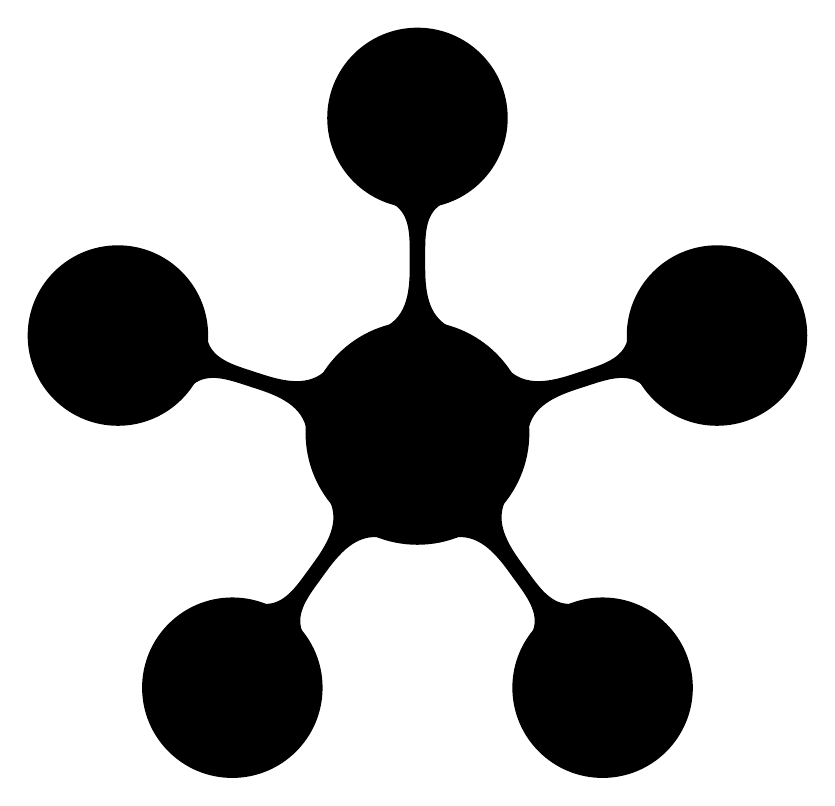
\begin{tikzpicture}[scale=0.8]
		\path[mindmap,level 1 concept/.append style=
				{sibling angle=72}]
		node[concept,scale=0.7] {\textbf{Benaderen}}
		[clockwise from=90]
		child { node[concept] {Waarom} }
		child { node[concept] {Wat discreet} }
		child { node[concept] {Waarmee} }
		child { node[concept] {Criterium} }
		child { node[concept] {Hoe} };
	\end{tikzpicture}
	\caption{Situering}
	\label{fig:Situering}
\end{figure}

\begin{description}
	\item [Wat] functies continu, discreet 1D/2D/3D
	\item [Waarmee] Veeltermen, trigonometrische functies, splines (veeltermen die aan elkaar vastgangen) basis van tekenprogramma's/tekenfilms, rationale functies, wavelets (compressie in de digitale beeldverwerking, wordt niet besproken in deze cursus), neurale netwerken, support vector machine.
	\item [Criterium] Hoe ga je de kwaliteit van zo een benadering evalueren. Een maatstaf nodig, om te zeggen welk van de 2 benadering beter is (= de kwaliteit van de benadering). Bv kleinste kwadratenbenadering, minimax, Tayler expantie, interpolatie,...
	\item [Hoe]
	\item [Waarom] Compressie beeld, dominante periode te herkennen, beeld restoratie, ruis reductie, parameters in wiskunde model te identificeren.
\end{description}

\subsection{Voorbeeld: benadering van een continue functie}
"Bepaal een veeltermbenadering van graad 4 voor de functie $e^x$ over $[-1,1]$."

\begin{exam} Bespreek het opstellen van een n-de graads Taylor-, interpolatie- en kleinstekwadraten veelterm benadering voor een continue functie f(x) op het interval [a,b]. Hoe stel je de benadering op? Hoe ziet de foutenkromme er uit? Wat zijn de voor- en nadelen van de methodes? Bewijs de stelling over het aantal en de ligging van de nulpunten van de foutenkromme bij de kleinste-kwadratenbenadering. Waarom is de kennis van de nulpunten nuttig? Welk van die methodes zijn bruikbaar voor het benaderen van een discrete functie? Bijvragen: Geef andere voorbeelden van interpolatieveeltermen? (Newton, Vandermonde) Op welke manier wordt de kleinste kwadratenvergelijking opgelost voor continue functies? (Normaalstelsel) Hoe evalueer je de nulpunten van de benaderende fout $r_n = phi_{n+1}(x)$? (Eigenwaarden van tridiagonaalmatrix alpha, nu, lambda)
	\begin{description}
		\item [Taylor-ontwikkeling] in $x=0$ (dus Maclaurin)
		      Functiewaarden in punt 0 alsook van 1 tot 4de orde afgeleide. Onder alle veeltermen is dit de veelterm die het meeste afgeleiden gemeenschappelijk heeft.
		      ${\displaystyle f(x)=f(a)+{\frac {f'(a)}{1!}}(x-a)+{\frac {f''(a)}{2!}}(x-a)^{2}+{\frac {f^{(3)}(a)}{3!}}(x-a)^{3}+\ldots =\sum _{n=0}^{\infty }{\frac {f^{(n)}(a)}{n!}}\,(x-a)^{n}}$

		      ${\displaystyle y_4(x) = 1+x+{\tfrac {1}{2}}x^{2}+{\tfrac {1}{3}}x^{3}+{\tfrac {1}{4}}x^{4} \!}$

		      $ r(s) (residu) = e^x - y_4(x) $

		      Nadeel
		      \begin{itemize}
			      \item  Exact in 0, een fout die heel traag stijgt en het grootst aan de randen, Foutenkromme ongelijkmatig verdeelt, randen $10^-2$ en in center $10^-7$. Liever foutenkromme evenwichtiger.
			      \item Fout kleiner maken door meer termen te nemen, maar dan ben je nog nauwkeuriger in het midden waar je al nauwkeurig genoeg bent.
			      \item Echt veel termen moet meenemen, bij $e^x$ wordt het snel heel klein, elke bijkomende term is veel kleiner als de laatste term, de fout die gemaakt wordt is gelijk aan de eerste term die verwaarloost wordt. Bij $ln(1+x)$ is een Taylor ontwikkeling die heel traag converteert, echt veel termen (termen blijven lang groot) nodig om een bepaalde nauwkeurigheid te bekomen. $ln(1+x) = x - \frac{x^2}{2}+ \frac{x^3}{3}+ \frac{x^4}{4}+ \frac{x^5}{5}$
		      \end{itemize}
		      \begin{figure}[!h]
			      \centering
			      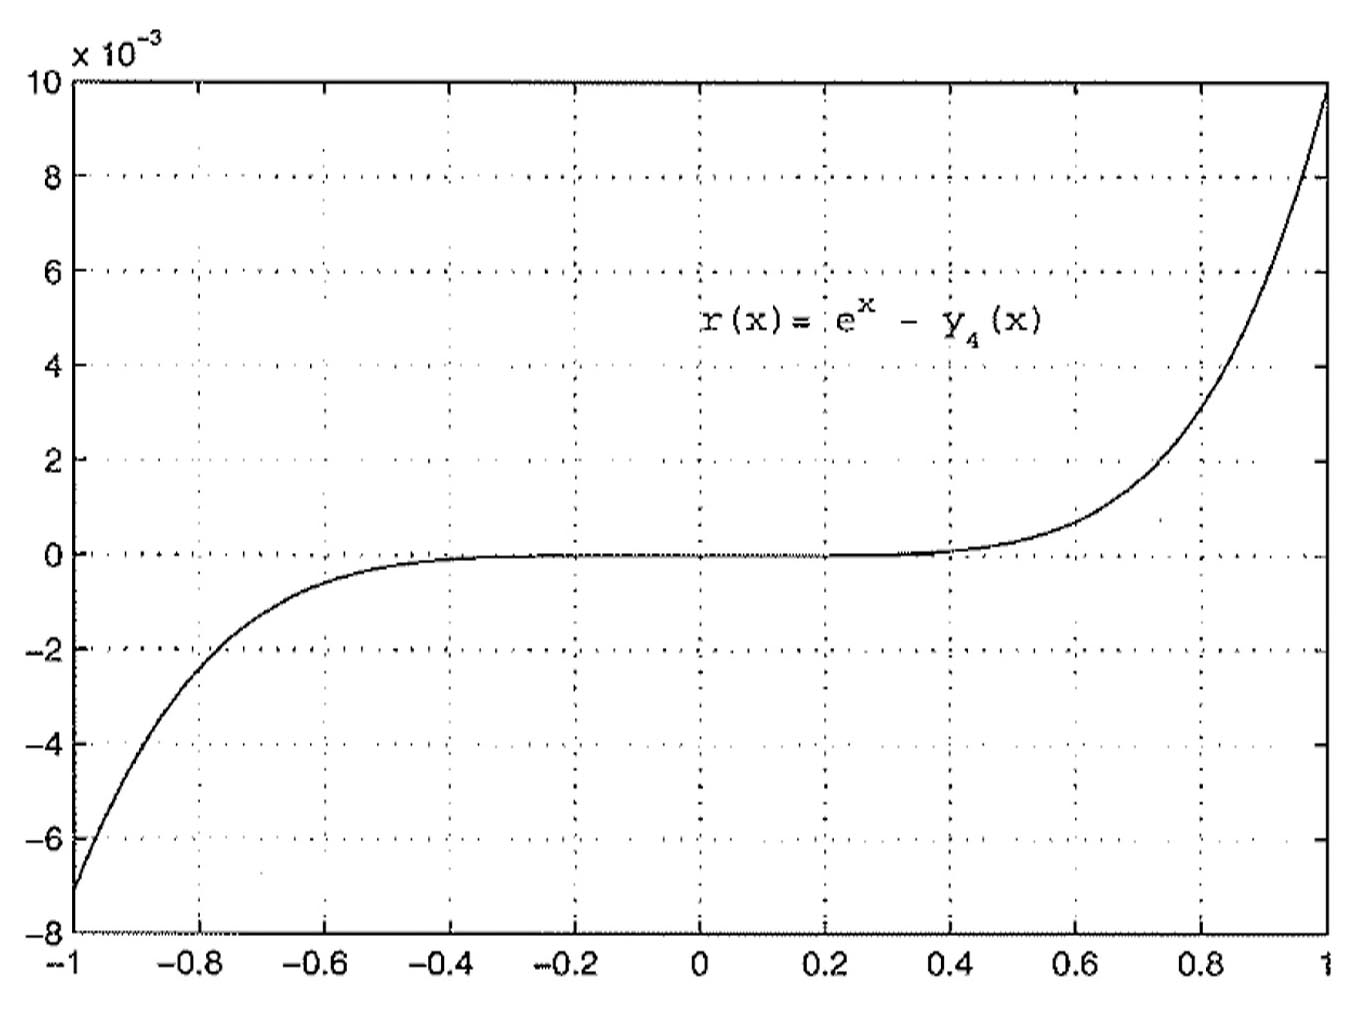
\includegraphics[width=0.5\textwidth]{FoutMaclaurinBenadering}
			      \caption{Fout van de Maclaurin-benadering van graad 4 voor $e^x$}
		      \end{figure}

		\item [Interpolatie] kies een aantal punten, veelterm graad 4 $\rightarrow$ 5 punten nodig van $x_1$ tot $x_5$, mag equidistant liggen of meer geclusterd. Deze punten berekenen op 1 of andere manier (natuurlijk niet met de routine die we nu aan het opstellen zijn), bv Taylor ontwikkeling met 100 termen, veel werk maar niet erg. Belangrijk dat het gebruik heel snel kan.
		      Zodat de veelterm $y_4(x)$ de juiste functiewaarden aanneemt in deze 5 punten (unieke oplossing).
		      Keuze: hoe veeltermen voorstellen? Welk rekenwerk je hebt.
		      Methode:
		      \begin{description}
			      \item [Vandermonde] (monomiale basis) $y_4(x)=a_0+a_1 x+a_2 x^2+a_3 x^3+a_4 x^4$ en eis dat $y_4(x_1) = e^{x_1} ,  y_4(x_2) = e^{x_2},y_4(x_3) = e^{x_3},y_4(x_4) = e^{x_4},y_4(x_5) = e^{x_5}$  $\rightarrow$ stelsel \\ Matrix:
			            ${\begin{bmatrix}1&x_{0}&x_{0}^{2}&\ldots &x_{0}^{n}\\1&x_{1}&x_{1}^{2}&\ldots &x_{1}^{n}\\\vdots &\vdots &\vdots &&\vdots \\1&x_{n}&x_{n}^{2}&\ldots &x_{n}^{n}\\\end{bmatrix}}{\begin{bmatrix}a_{0}\\a_{1}\\\vdots \\a_{n}\end{bmatrix}}={\begin{bmatrix}y_{0}\\y_{1}\\\vdots \\y_{n}\end{bmatrix}}.$
			      \item [Newton]  $y_4(x)=a_0+a_1(x-x_1)+a_2(x-x_1)(x-x_2)+a_3(x-x_1)(x-x_2)(x-x_3)+a_4(x-x_1)(x-x_2)(x-x_3)(x-x_4)$
			            Voordeel $a_k$ zonder stelsel op te lossen, via gedeelde differenties.
			      \item [Lagrange]  \begin{form}
				            $y_4(x):=\sum _{k=1}^{5}e^{xk}l_k(x)$
			            \end{form}
			            Geeft een expliciete oplossing, geen rekenwerk meer. Gemakkelijk op te stellen moeilijk te evalueren. Veelterm wordt geschreven als een lineaire combinatie van de functiewaarden $e^{xk}$ (gekende getallen) met de basisfuncties (functies veelterm van graad 4 zodat $l_i(x_j)$ = 0 indien i $i \neq j$ en 1 indien $i=j$
			            \\
			            \begin{form}
				            $l_k(x)={\frac {(x-x_{0})}{(x_{k}-x_{0})}}\cdots {\frac {(x-x_{k-1})}{(x_{k}-x_{k-1})}}{\frac {(x-x_{k+1})}{(x_{k}-x_{k+1})}}\cdots {\frac {(x-x_{N})}{(x_{k}-x_{N})}}$
			            \end{form}
		      \end{description}
		      $ r(s) (residu) = e^x - y_4(x) $
		      Residu 0 in de meetpunten. Punten wat verschuiven verandert de foutencurve. Foutencurve overal even groot.
		      Nadeel, moeilijk om de punten te selecteren. Waar kies je de punten? Functie ergens lokaal vreemde vorm? Wat als we hier geen punten zetten, dan mist men deze vorm. Nog een nadeel opstellen zorgt voor afrondingsfouten. Veeltermco\"effici\"enten gevoelig voor afrondingsfouten.

		      \begin{figure}[h]
			      \centering
			      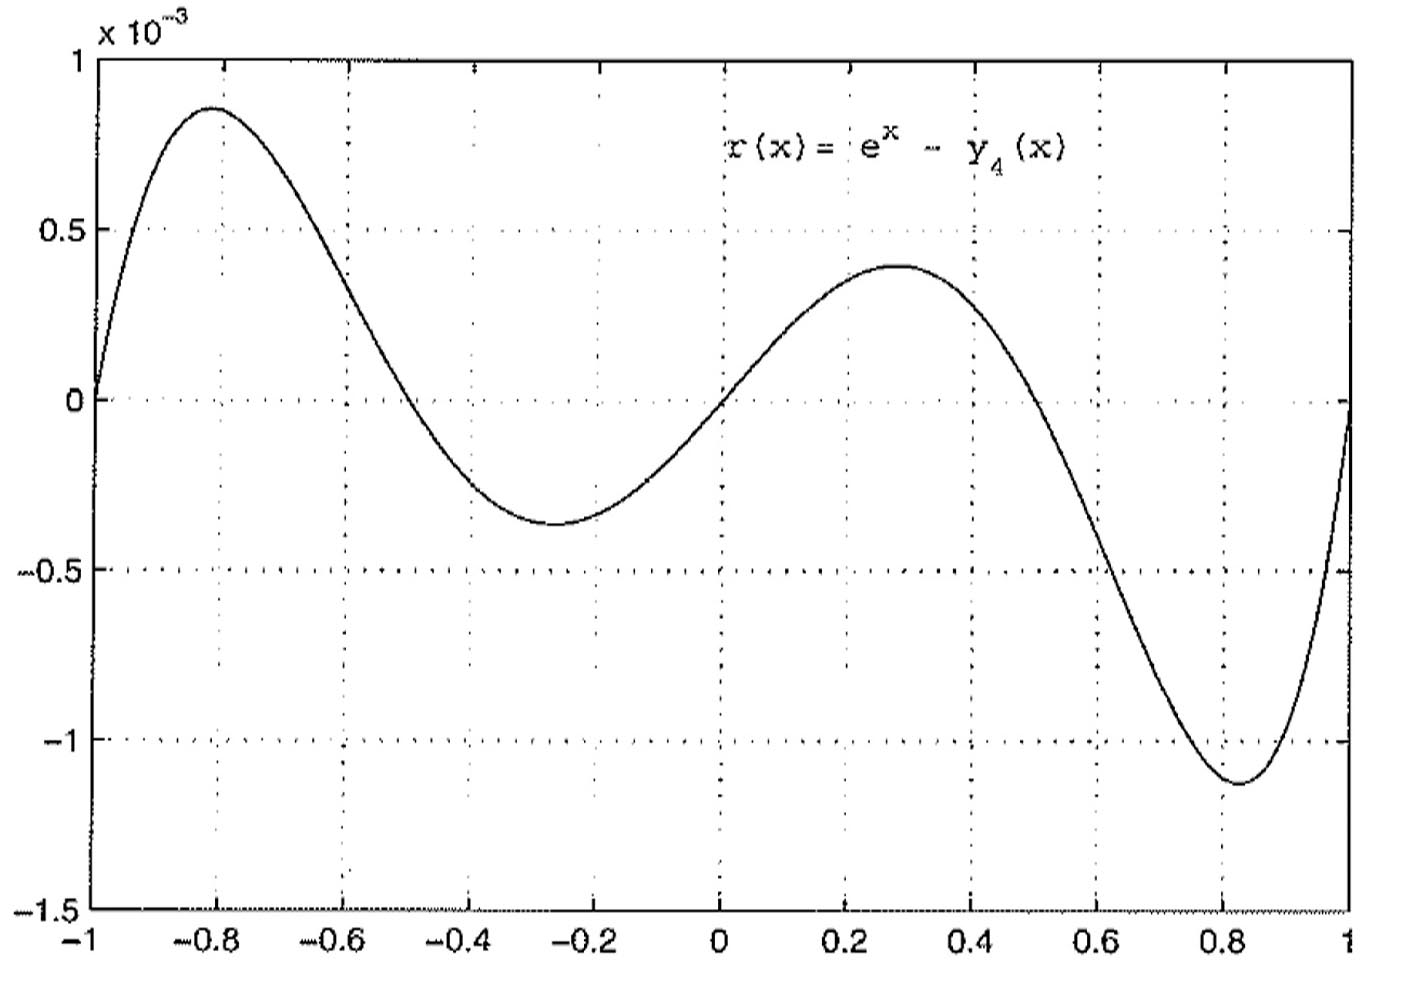
\includegraphics[width=0.5\textwidth]{FoutInterpolerendeBenadering}
			      \caption{Fout van een interpolerende benadering van graad 4 voor $e^x$}
		      \end{figure}

		\item [Minimax] verschil met vorige, hier houdt men rekening met volledige functie/interval, waardoor we geen lokale pieken/singulariteiten missen.
		      $y_4(x) = \underset{y_4\in P_4[-1,1]}{\operatorname {arg\,min}}\underset{x\in [-1;1]}{\operatorname {max}}|e^x - y_4(x)|$
		      Veelterm van graad 4, 5 co\"effici\"enten, element van 5 dimensionale ruimte, zoek maximum in absolute waarde in interval $[-1;1]$, is een getal dat we willen minimaliseren, zoek minimum in de verzameling van alle veeltermen van $y_4$ die behoren tot de ruimte van de veelterm die gaat van $[-1;1]$. De gezochte veelterm is waar het maximum geminimaliseerd wordt. Is een optimalisatiecriterium in een 5 dimensionale ruimte.

		\item [Kleinste kwadraten] Ook een optimalisatie probleem, maar nu afwijking tussen benadering en de te benaderen functie anders formuleren. Verschil met mini max, nu wel makkelijk uit te rekenen
		      $y_4(x) = \underset{y_4\in P_4[-1,1]}{\operatorname {arg\,min}} \int_{-1}^1 w(x) (e^x-y_4(x))^2 dx $

		      Keuze $w(x)$ geeft aan waar je fout liefst kleinst wilt hebben, gewichtsfunctie \\
		      $w(x) \equiv 1 \rightarrow$ legendre \\
		      $w(x) = \frac{1}{\sqrt{1-x}} \rightarrow $ chebyshev, randen oneindig veel gewicht
		      \begin{figure}[h]
			      \centering
			      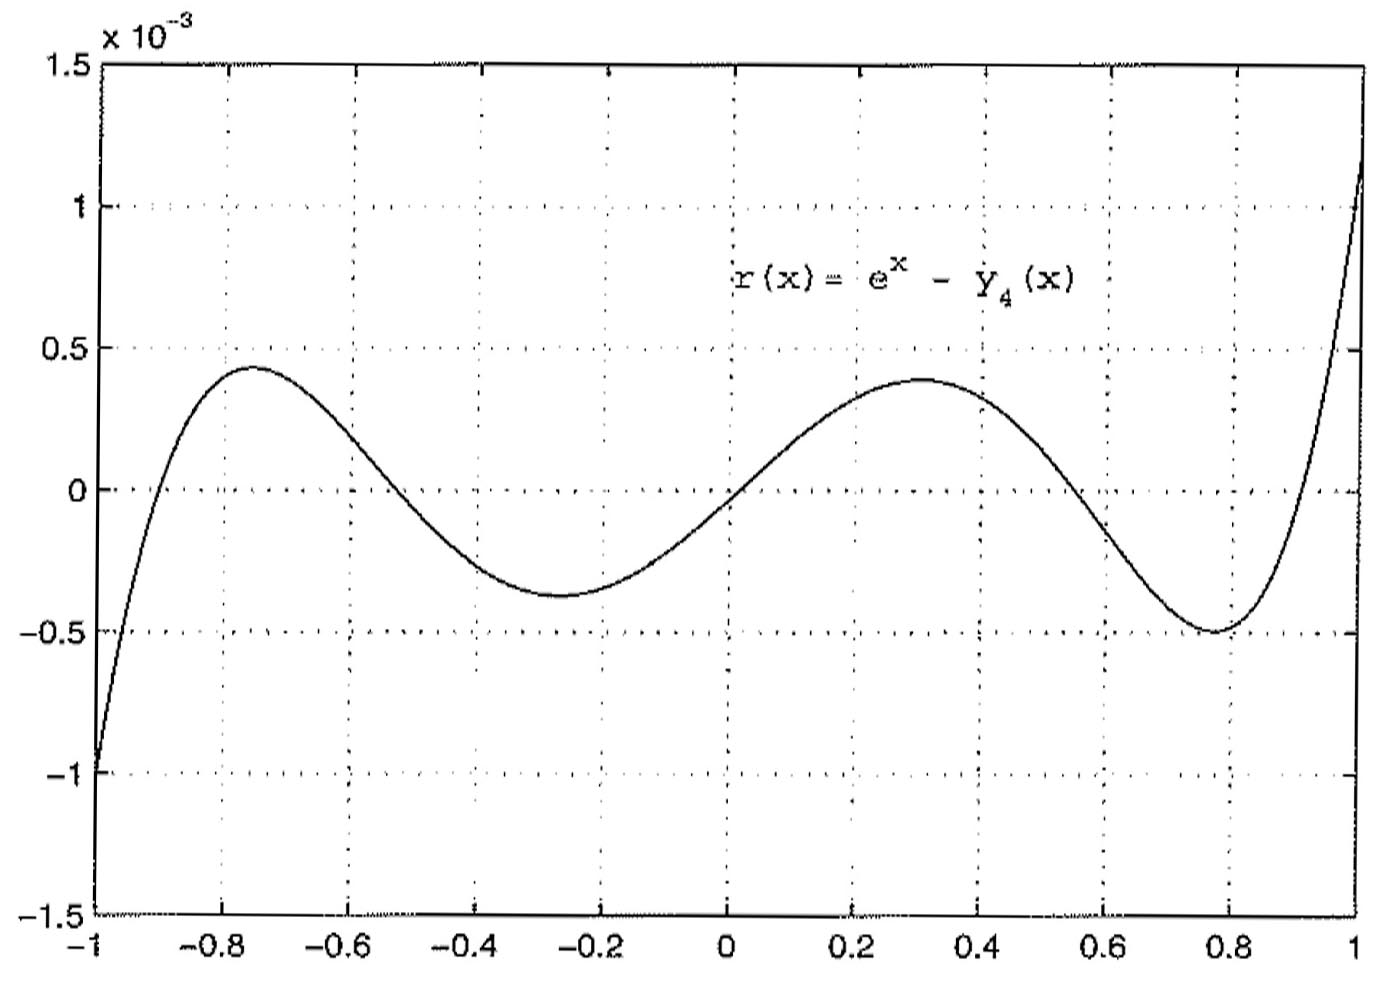
\includegraphics[width=0.5\textwidth]{FoutKleinsteKwadratenLegenreBenadering}
			      \caption{Fout van een kleinste-kwadraten benadering van graad 4 voor $e^x$ met $w(x)\equiv 1$}
		      \end{figure}
		      \begin{figure}[h]
			      \centering
			      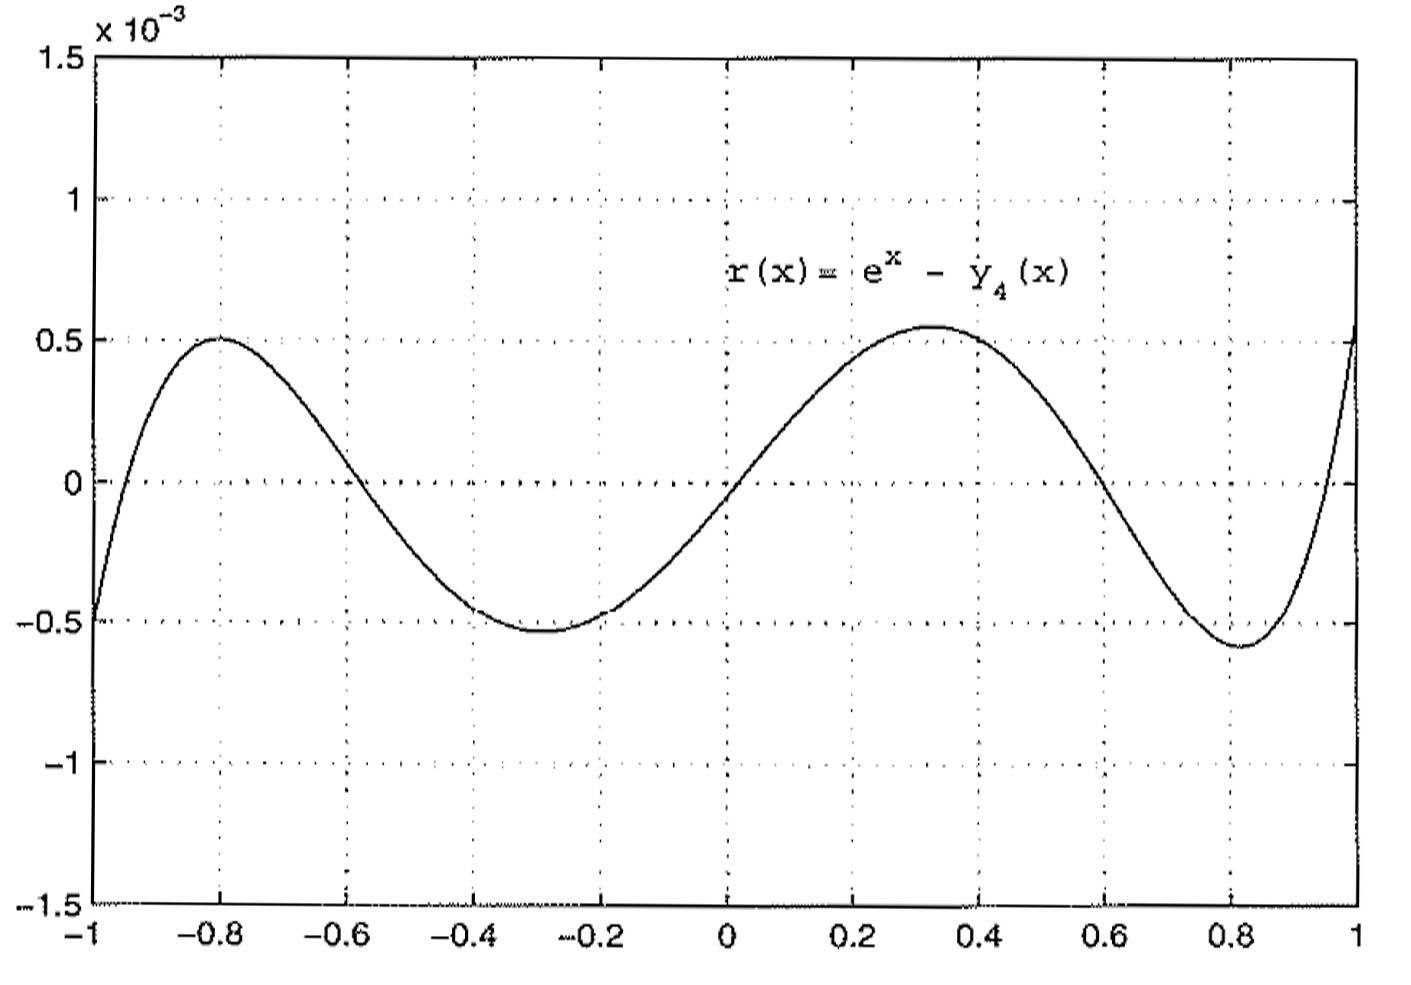
\includegraphics[width=0.5\textwidth]{FoutKleinsteKwadratenChebyshevBenadering}
			      \caption{Fout van een kleinste-kwadraten benadering van graad 4 voor $e^x$ met $w(x)=\frac{1}{\sqrt{1-x}}$}
		      \end{figure}
	\end{description}

	\subsection{Voorbeeld: benaderen discrete functie}
	Zoek een veelterm die goed aansluit bij de dingen je opgemeten hebt.
	\begin{description}
		\item[Taylor-ontwikkeling] NIET Afgeleide nodig, van continue functie hier niet
		\item[Interpolatie] NIET Geen reden om exact door de punten te gaan. Of als je miljoen punten hebt dan benadering van veelterm graad miljoen, niet te evalueren. Welke punten selecteren en hoeveel?
		\item[Minimax]  $y_n(x) = \underset{y\in P_n}{\operatorname {arg\,min}}\underset{i=1,\ldots,N}{\operatorname {max}}|f_i - y(x_i)|$
		      Als meetwaarden vrij nauwkeurig is, anders vermenigvuldigen met $\frac{1}{meetfout}$
		\item[Kleinste kwadraten]
		      $y_4(x) = \underset{y\in P_n }{\operatorname {arg\,min}} \sum_{-1}^1 w(x) (f_i-y(x))^2 dx $
	\end{description}
\end{exam}

\subsection{Keuze benaderingsfuncties}
Waarmee ga je benaderen? Veelterm niet altijd geschikt, altijd oneindig links en rechts dan komt ie naar de oorsprong schommelt een paar keer en dan naar oneindig. Niet alles wat we willen benaderen heeft deze vorm.
Onze (lineaire) benadering zal altijd combinatie zijn van gekende functies en de co\"effici\"enten.
$y(x)=\sum_{k=0} a_k \phi_k(n)$ waar $ \phi_k(n)$ gekend is.
\\\\
Waarom andere basissen:
\begin{itemize}
	\item eenvoud
	\item vorm
	\item fysische toepassing
	\item numeriek, nauwkeurigheid (afrondingsfouten, conditiegetal bij veeltermen, zeker bij monomiale basis zeer slecht)
\end{itemize}
\chapter{Benaderingstheorie (les 1 en 2)}
\section{Overzicht}
\begin{figure}[h]
	\centering
	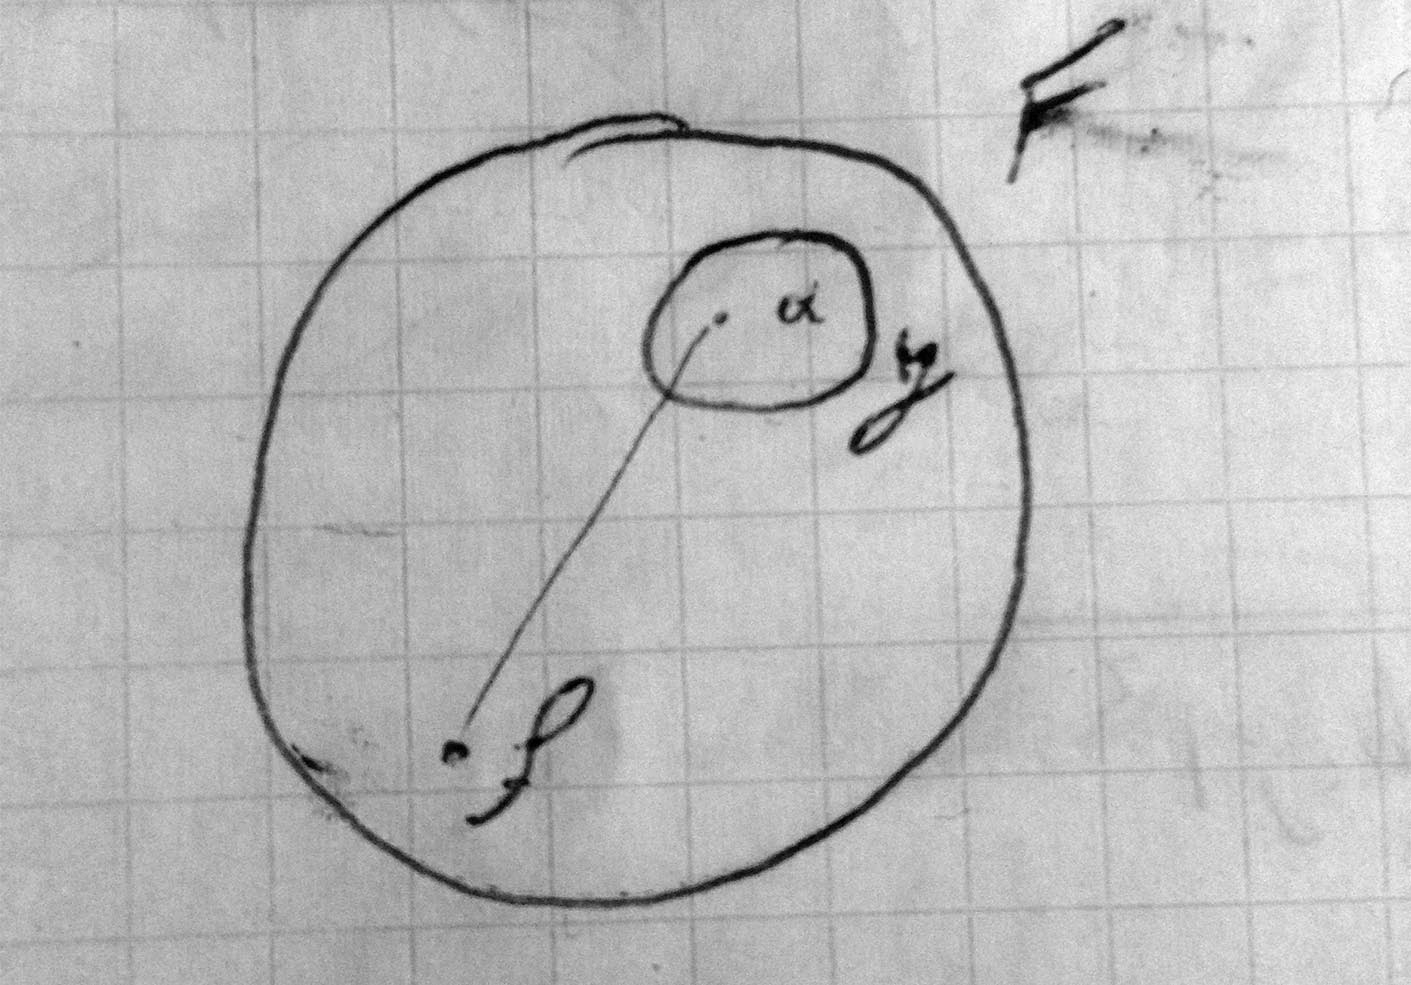
\includegraphics[width=0.5\textwidth]{Benaderingstheorie}
	\caption{Benaderingstheorie}
\end{figure}
$ F = C[-1,1] $ verzameling continue functies op -1,1 en $ y = P_4[-1,1]$ verzameling van veeltermen met graad 4 of minder op -1,1. f functie dat we willen benaderen.

\begin{exam}[Geef de definitie van een metrische, genormeerde, strikt genormeerde, unitaire en euclidische ruimte. Geef het verband tussen deze verschillende ruimten. Wat zijn de verbanden hiertussen?  Welke ruimte wordt C{[a,b]} met  de L2-afstand, de triviale afstand, de max-afstand. Bespreek het belang van deze ruimten in de benaderingstheorie]   

Aan de verzameling F een bepaalde structuur/eigenschappen opleggen. Hoe meer eigenschappen hoe meer dingen aantonen/analyseren:
\begin{description}
\item[Metrische ruimte $\rho(x,y)$] afstand meten tussen 2 punten. Beste benadering defini\"eren alsook de existentie / bestaans vraag.
\item[Genormeerde ruimte $||\vec{x}||$] defini\"eren we norm / grootte, spreken we van grootte van de fout. Alsook aantal benaderingen, de uniciteit (= zijn er 1 of meer oplossingen). 
\item[Unitaire ruimte $( \vec{x},\vec{y} ) $] ruimte met scalair product, loodrechte stand (orthogonaliteit) en strict genormeerd. Uitspraak over karakteristiek, weet je waar beste benadering ligt? Naarlaten van een loodlijn op de benaderingsruimte (de orthogonale projectie).
\item[Euclidische ruimte] is een unitaire ruimte met een eindige dimensie, je hebt een basis, je kan een punt kenmerken door een paar getallen. Algoritme / berekening.
\end{description}
\end{exam}

 \begin{figure}[h]
 \centering
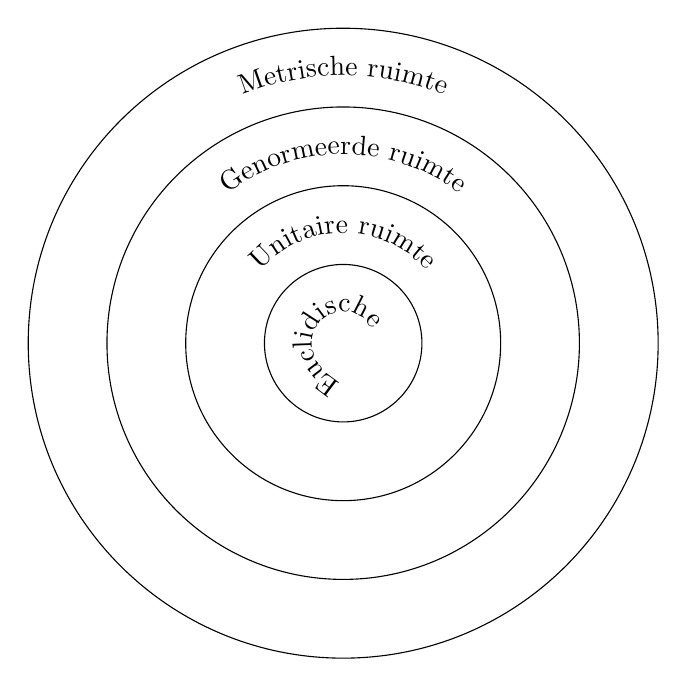
\begin{tikzpicture}
\coordinate (O) at (0,0);
\foreach \j in {1,...,4} \draw (O) circle (5-\j);
\foreach \k/\text in {0/Metrische ruimte,1/Genormeerde ruimte,2/Unitaire ruimte,3/Euclidische ruite} \draw[decoration={text along path,reverse path,text align={align=center},text={\text}},decorate] (3.4-\k,0) arc (0:180:3.4-\k);
\begin{scope}[xshift=6cm]
\end{scope}
\end{tikzpicture}
  \caption{Onion ruimtes}
  \end{figure}

\section{Metrische ruimte $\rho(x,y)$}
Metriek / afstandsfunctie $\rho (x,y) $ met $ \rho : A x A \rightarrow \mathbb{R} $  
\begin{enumerate}
\item $\rho (x,y) \geq 0 $ positief 
\item $\rho (x,y) = 0 \Leftrightarrow x=y $ definiet
\item $\rho (x,y)=\rho(y,x) $ symmetrie
\item $\rho (x,y) \leq \rho(z,x)+\rho(z,y) $ driehoeksongelijkheid
\end{enumerate}
De eerste en derde kunnen afgeleid worden uit de anderen.

De afstand gedefinieerd als: $\rho(x,D) = \inf \left\{\rho(x,y)| y \in D\right\}$
Infimum omdat kleinste niet altijd bestat.

d is 'een' (er kan meer als 1 bestaan, bv cirkel) beste benadering in d voor x als: $\rho(x,d) = \rho(x,D) $. Een beste benadering bestaat niet altijd. 

\subsection{Voorbeelden}
\begin{description}
\item[Niet-klassieke]

\begin{description}
\item[Chordale afstand in $\mathbb{C}$]
De riemann bol, door de noordpool te verbinden met punt $z$, verkrijgt men een nieuw punt waar het de bol snijdt, de chordale afstand is de afstand tussen de nieuwe verkregen punten op de bol. \\
$\rho(0,noordpool) = \infty$ \\
$\rho(0,zuidpool) = oorsprong$ \\
$\rho(0,\infty) = 2$ \\
$\rho(0,1) = \sqrt{2}$ 
\item[Triviale afstand] Altijd 1 behalve als deze 0 moet zijn. Enkel in theorie gebruikt, om stellingen te ontkrachten. \\
$ \rho(x,y)=1 \,als\, x \neq y$ $\rho(0,\infty)=1 $\\ 
$ \rho(x,y)=0 \,als\, x=y$ $ \rho(0,0(0,1)) = 1 $
\item[Silvermanafstand] $\rho(A,B) = \#A \Delta B = \#(A \cup B) \setminus (A \cap B) $ Geeft de mate nabijheid van 2 groepen van studenten. 0 als groepen volledig overlappen.
\item[Hamming afstand] $\rho(0|0||,||00|)=2$
\item[Frobenius afstand] Geeft de mate van nabijheid tussen 2 matrixen weer. $\sqrt{\sum_i sum_j | a_{ij} - b_{ij}|^2}$

\begin{figure}[h]
	\centering
	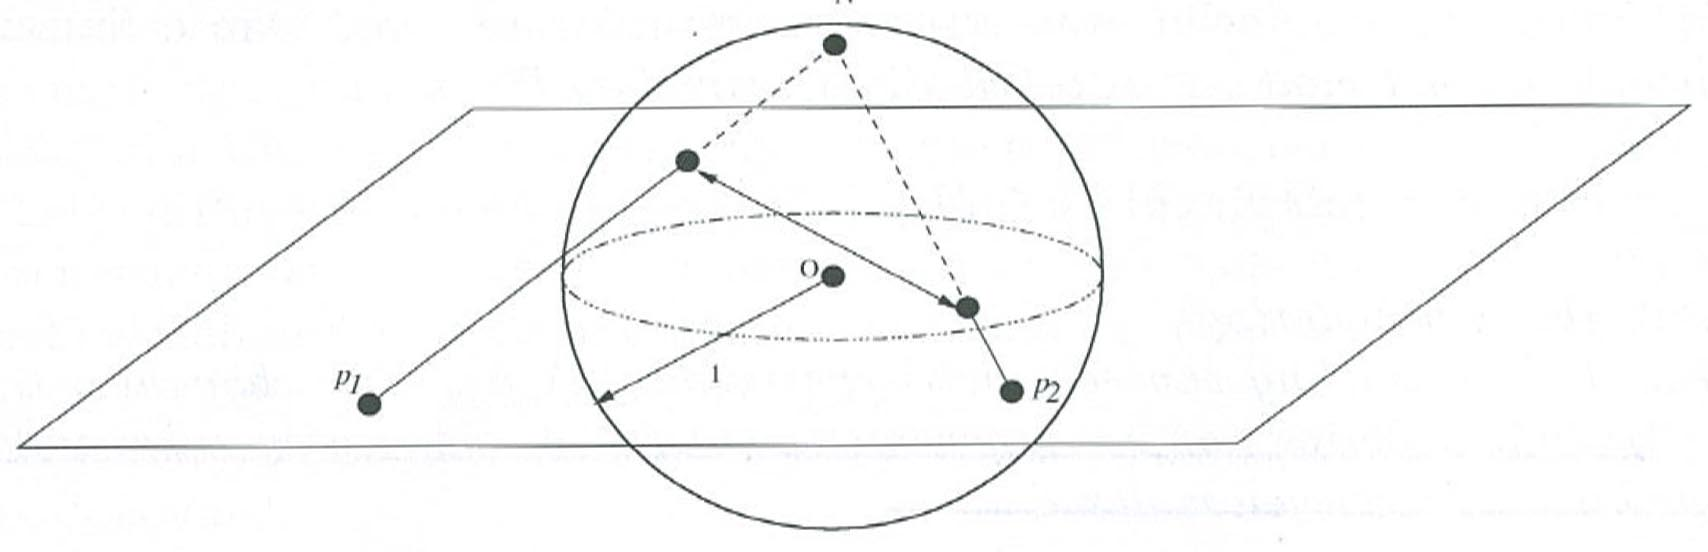
\includegraphics[width=0.5\textwidth]{ChordaleAfstand}
	\caption{Chordale afstand tussen punten $p_1$ en, $p_2$}
\end{figure}
\end{description}

\item[in continue functieruimten] $C[a,b]$
\begin{description}
\item[$L_\infty$-afstand] of max-afstand (gebruikt in minimax benadering): $\underset{x\in [a;b]}{\operatorname {max}}|f(x)-g(x)|=\rho(f,g) $\\
Check voorwaarden afstand: \\
$ f(x)-g(x)=f(x)-h(x)+h(x)-g(x)$ \\
$ |f(x)-g(x)| \leq|f(x)-h(x)|+ |h(x)-g(x)| $ \\
$\operatorname {max} |f(x)-g(x)| \leq \operatorname {max} |f(x)-h(x)|+ \operatorname {max} |h(x)-g(x)| $ \\
$\rho(f,g) \leq \rho(f,h)+\rho(h,g) $

\item[$L_p$ afstand] 
\begin{exam}$L_2[0, 1]$
$L_p[a,b]$ verzameling van functieklassen (functies die bijna overal gelijk zijn) die ook discontinue functies toelaat uitbreiding van $C[a,b]$. Verzameling van alle functies, waarvoor geldt dat $\sqrt[p]{\int_a^b w(x)|f(x)-g(x)|^p dx}$ aan alle voorwaarden voor een afstand voldoet, met $p \geq 1$ om aan laatste voorwaarde te voldoen. \\
$f=g \iff f(x)=g(x)$ b.o. (bijna overal of a.e. almost everywhere)
$\rho(f,g)=0$ en toch $f\neq g$. We maken geen onderscheid tussen functie $f$ en $g$ die bijna overal gelijk zijn. Wat is bijna overal? Dit is een term afkomstig uit de maattheorie, waarmee bedoeld wordt: overal behalve op een voor de theorie verwaarloosbaar deel, een verzameling van maat nul. Dit kan men zien als een lintje nemen van $\epsilon$ lengte, kunnen we dit verknippen en elk van deze punten bedekken? Bv rationele punten, dit is oneindig aftelbaar (men kan ze opsommen, oneindig veel) waardoor we steeds een kleiner stukje lint kunnen nemen $\frac{\epsilon}{2}$,$\frac{\epsilon}{4}$,$\frac{\epsilon}{8}$,\ldots\\ (We moeten integraal ook aanpassen van Rieman naar Libesque integraal.)
\textbf{$L_2$} kleinste kwadratenbenadering %TODO meer info? Examenvraag
\end{exam}
\end{description}
\item[in discrete functieruimten] 
\begin{description}
\item[Eindige dimensie] Aantal losse punten, $x_1,x_2,\ldots,x_n$ Verzameling van al discrete functies, vectoren van functiewaarden. $\mathbb{R}^N$ of $\mathbb{C}^N$, Vectoren van lengte N
\item[Oneindige dimensie] $l_p(\mathbb{R}), l_p(\mathbb{C})$ \\
$l_p = \sum_{i=1}^N w_i |f_i-g_i |^P < \infty $ \\
$l_\infty = \underset{i=1,\ldots,N}{\operatorname{max}} |f_i-g_i|$
\end{description} 
\end{description}

\section{Genormeerde ruimte $||\vec{x}||$}
\begin{enumerate}
\item $||\vec{x}|| \geq 0 $ positief definiete functionaal
\item $||\vec{x}|| = 0  \iff \vec{x} = \vec{0} $ positief definiete functionaal
\item $||a \vec{x}|| = |a| \cdot ||\vec{x}|| $ homogeniteitseigenschap
\item $||\vec{x}+\vec{y}|| \leq ||\vec{x}|| + ||\vec{y}|| $ driehoeksongelijkheid
\end{enumerate}
Door $\vec{y} = \vec{-x}$ bekomt men van 4de voorwaarde ook de 1ste voorwaarde. $||\vec{x}-\vec{x}|| \leq ||\vec{x}|| + ||\vec{-x}|| $ \\
$||0|| \leq ||\vec{x}|| + ||\vec{-x}|| $

\begin{enumerate}
\item Een genormeerde ruimte is ook metrisch \\
$||\vec{x}-\vec{y}||$ is een afstand $\rho(x,y)$
\item Zij $(a,\rho)$ een metrische vector ruimte dan is $\rho(\vec{0},\vec{x})$ een norm $\iff$
\begin{enumerate}
\item $\rho(\vec{x},\vec{y})=\rho(\vec{x}+\vec{z},\vec{y}+\vec{z)}$ translatie-invariantie
\item $\rho(a\vec{x},a\vec{y})=a\rho(\vec{x},\vec{y}) $ voor a $\in \mathbb{R}^+ (a \geq 0)$  homogeen
\end{enumerate}
\end{enumerate}
De triviale afstand is niet homogeen. $\rho(x,y) = 1, x \neq y$, $\rho(x,y) = 0, x = y$ Wordt niet 2 indien we $a \rho(x,y,)$ met $x \neq y$.



\begin{figure}[h]
	\centering
	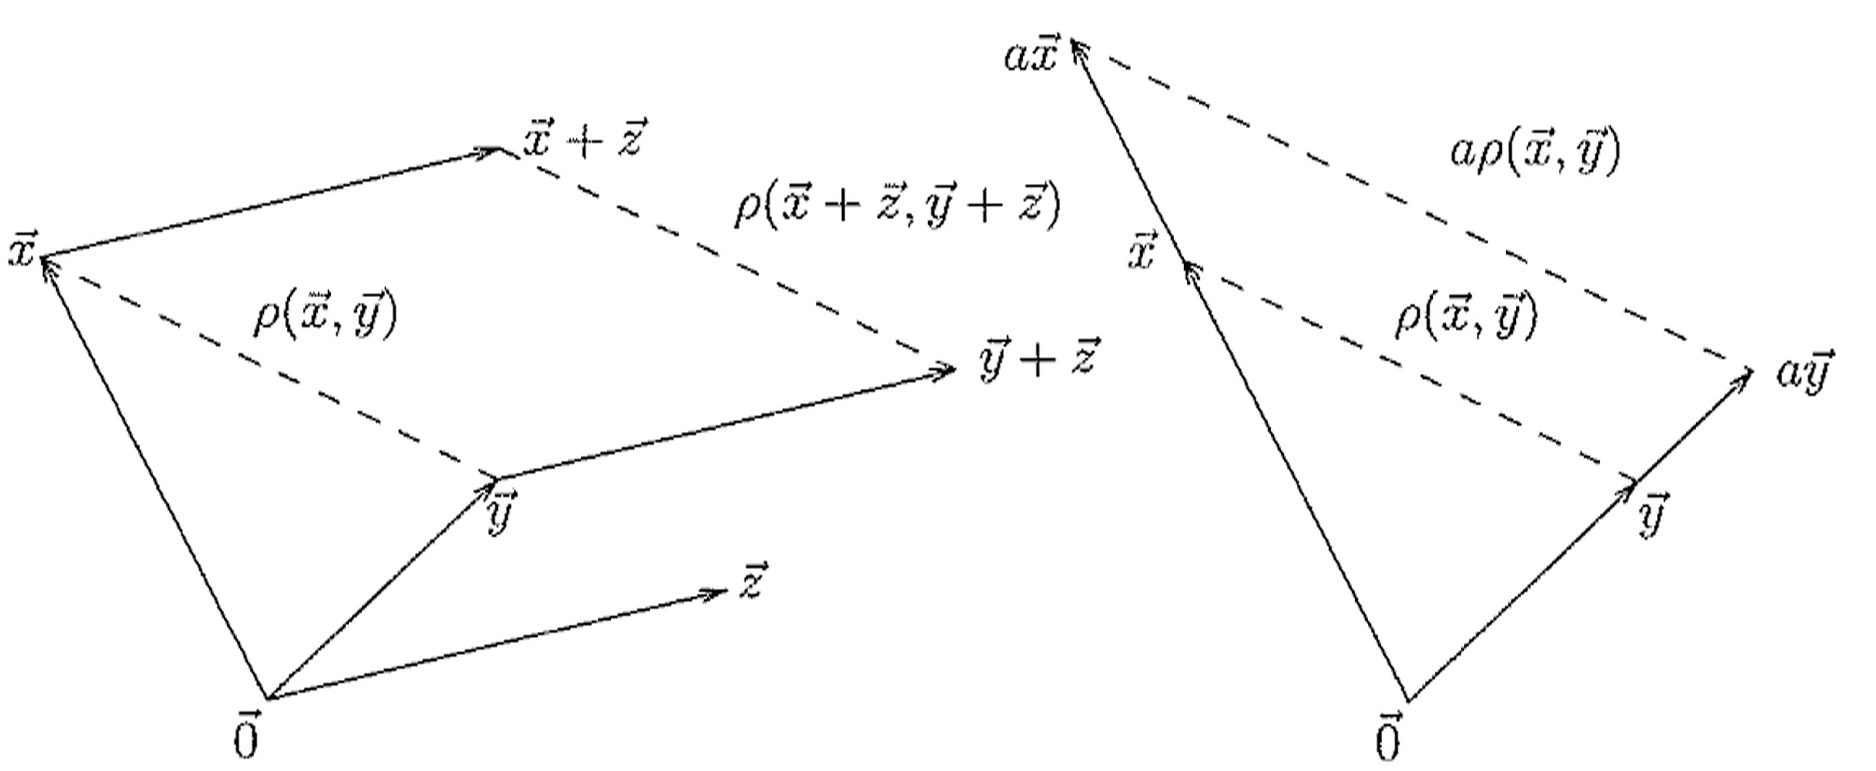
\includegraphics[width=0.5\textwidth]{TranslatieInvariantieHomogeniteitAfstandVectorruimte}
	\caption{Translatie-invariantie en homogeniteit van een afstand in een vectorruimte}
\end{figure}

\subsection{Voorbeelden}
\begin{description}
\item[B[a,b]] dit is de norm van de verzameling van continue functies op $[a,b]$ , $ \underset{x\in[a,b]}{\operatorname{sup}} |f(x)|$
$ |f(x)+g(x)| \leq |f(x)|+|g(x)| $ \\
$\operatorname {max}|f(x)+g(x)| \leq \operatorname {max}|f(x)|+ \operatorname {max} |g(x)| $
\item[$L_p$[a,b]] $\sqrt[p]{\int_a^b w(x)|f(x)|^p dx}=||f||_p$
\item[$\mathbb{R}^N,\mathbb{C}^N$] $\sqrt[p]{\sum_{i=1}^N w_i|f_i|^p dx}=||f||_p$
\end{description}

\subsection{Beste benadering}
$\tilde{B}(\vec{0},1)=\{(x,y)| \, ||(x,y)||=1\}$ of $\{\vec{x}| \, ||\vec{x}||=1\}$ \\
Al de punten liggen even ver naargelang de norm.
\begin{description}
\item [$l_2$] $\sqrt{x^2+y^2}=1$
\item[$l_1$] $|x|+|y|=1$
\item [$l_\infty$] $\operatorname{max}\{{|x|,|y|}\}=1$
\end{description}
\begin{figure}[h]
	\centering
	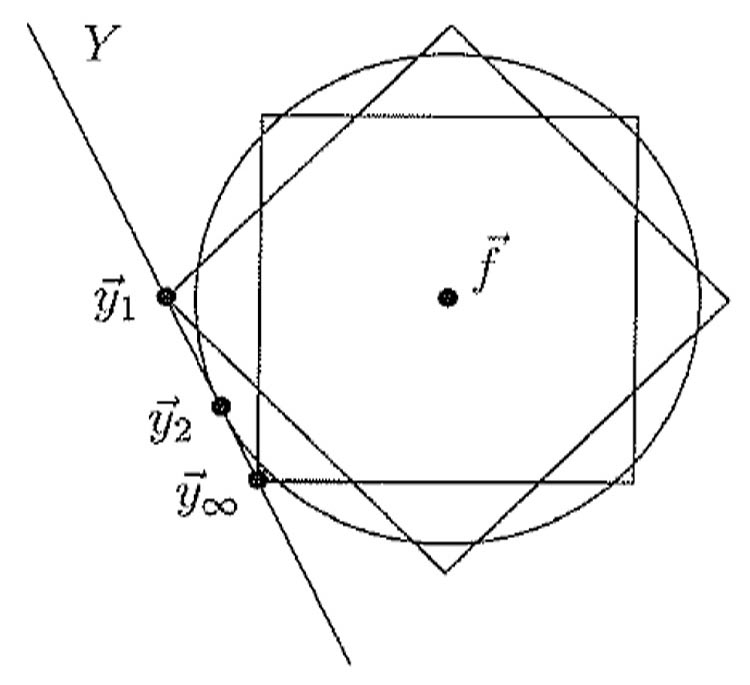
\includegraphics[width=0.5\textwidth]{BesteBenaderingPuntFVolgensNormen}
	\caption{Beste benadering voor het punt $\vec{f}$ volgens de 1-norm,2-norm,$\infty$-norm.}
\end{figure}
\begin{figure}[h]
	\centering
	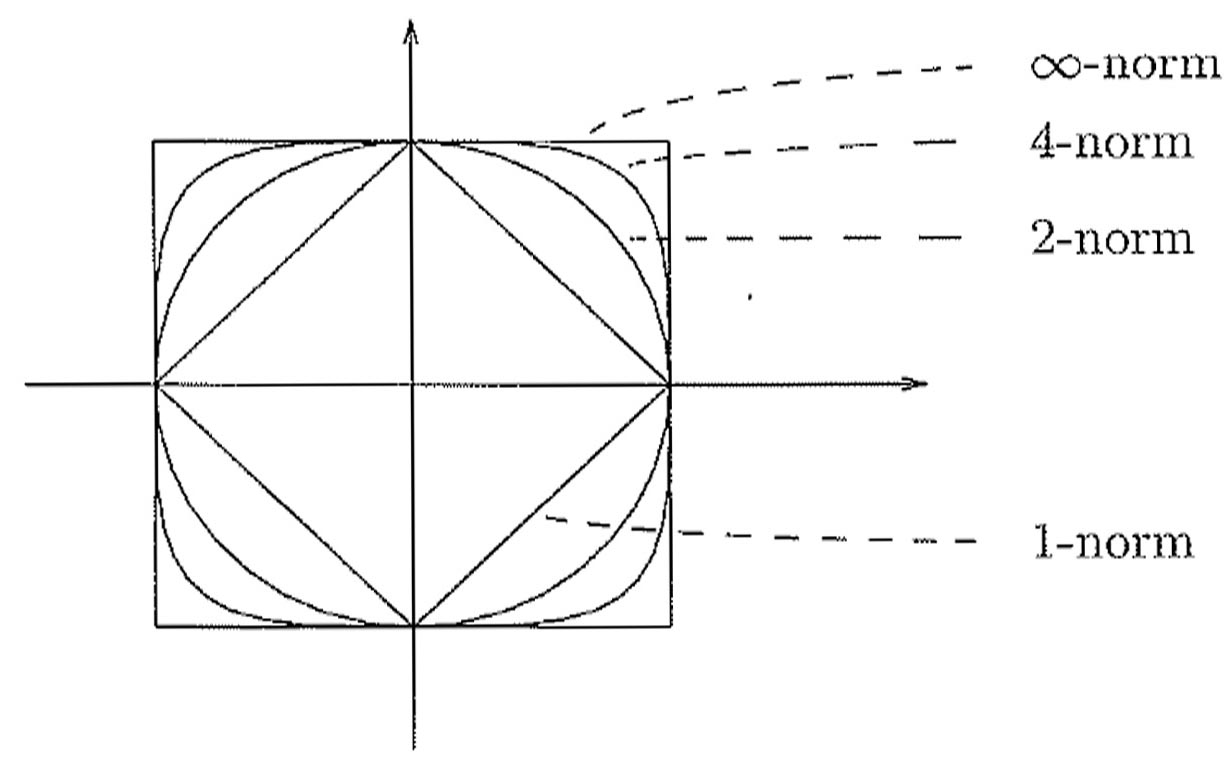
\includegraphics[width=0.5\textwidth]{EenheidscirkelsVlak}
	\caption{Eenheidscirkels in het vlak}
\end{figure}

Altijd maar 1 oplossing/punt als de bol strict convex is. Anders zou het kunnen zijn dat we oneindig veel oplossingen hebben.

\begin{figure}[h]
	\centering
	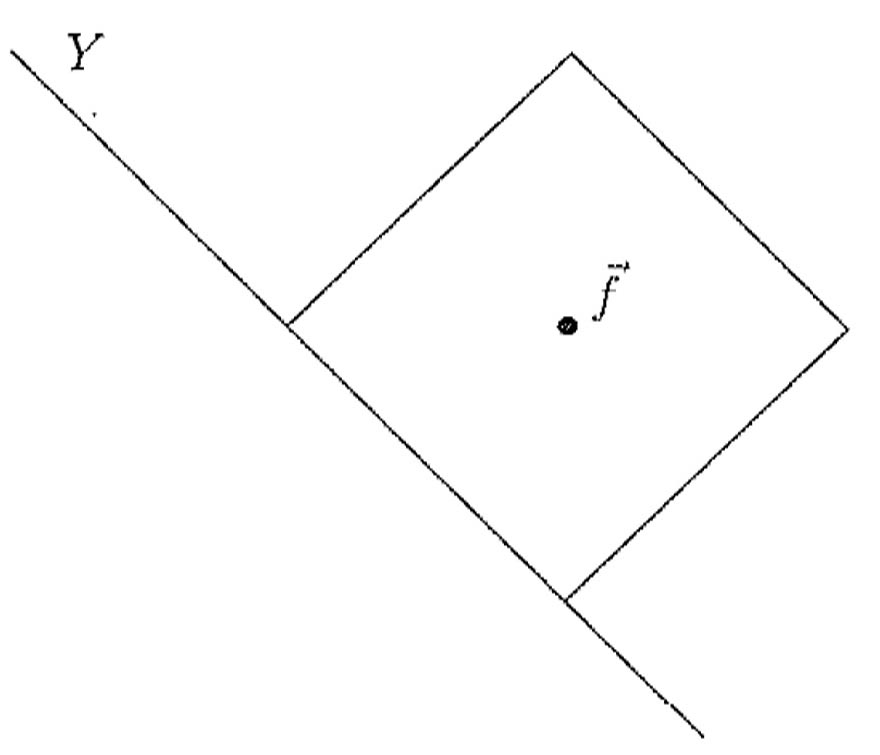
\includegraphics[width=0.5\textwidth]{MeervoudigheidBesteBenadering1Norm}
	\caption{Meervoudigheid van de beste benadering in de 1-norm}
\end{figure}

\subsection{Convexiteit} %TODO, wat aanvullen
\begin{exam} [Genormeerde ruimte, strikt genormeerde ruimte]
C is convex $\forall x_1,x_2 \in C: L(lijnstuk)(x_1,x_2) \in C $ \\
Waarom moet p steeds groter zijn als 1?
C is strict convex met $L(x_1,x_2)=\{\vec{x} | \vec{x} = \lambda \vec{x_1}+(1-\lambda) \vec{x_2} $ met $\lambda \in ((0,1) \}$ \\\\
$\vec{x_1},\vec{x_2} \in B(\vec{a},1)$ \\
$ ||\vec{a}-(\lambda\vec{x_1}+(1-\lambda)\vec{x_2})||=||\lambda\vec{a}-\lambda\vec{x_1}+(1-\lambda)\vec{a}-(1-\lambda)\vec{x_2}|| \leq |r|$ \\
$\lambda||\vec{a}-\vec{x_1}||+(1-\lambda)||\vec{a}-\vec{x_2}|| \leq r$ \\\\
$||\vec{x_1}|| = 1 = ||\vec{x_2}|| \rightarrow || \frac{x_1+x_2}{2} || <2 \rightarrow ||x_1+x_2||<2$
\end{exam}
\section{Unitaire ruimte $( \vec{x},\vec{y} ) $}
$(\cdot,\cdot):V*V \rightarrow \mathbb{R}$
\begin{enumerate}
\item $(a\vec{x},\vec{y})=a(\vec{x},\vec{y}$
\item $(\vec{x}+\vec{y}\vec{z})=(\vec{x},\vec{z})+(\vec{y},\vec{z})$
\item $(\vec{x},\vec{y})=(\vec{y},\vec{x})$ symmetrie
\item $(\vec{x},\vec{x}) > 0 \iff \vec{x} \neq \vec{0}$ definiet
\end{enumerate}
Aantal voorwaarden bij elkaar: $(\vec{x},a\vec{y})=\bar{a}(\vec{x},\vec{y})$

\subsection{Verband met vorige ruimte}
Cauchy-Schwarz $|(\vec{x},\vec{y})| \leq \sqrt{(\vec{x},\vec{x})}*\sqrt{(\vec{y},\vec{y})}$ \\
Te bewijzen: $\sqrt{(x+y,x+y)} \leq \sqrt{(x,x)}+\sqrt{(y,y)}$
\begin{enumerate}
\item Een unitaire ruimte is genormeerd $||\vec{x}||=\sqrt{(\vec{x},\vec{x})}$ is een norm.
\item Zij $(A,||\cdot||)$ een genormeerde ruimte dan geldt dat het unitair is als de norm voldoet aan de parallellogram gelijkheid. \\
\begin{form}
$ ||x+y||+||x-y||^2=2||x||^2+2||y||^2$ \\
$||\vec{x}|| = \sqrt{(\vec{x},\vec{x})}$
$(\vec{x},\vec{y})=1/4\{||x+y||^2-||x-y||^2\}$ is een scalair product.
\begin{figure}[h]
	\centering
	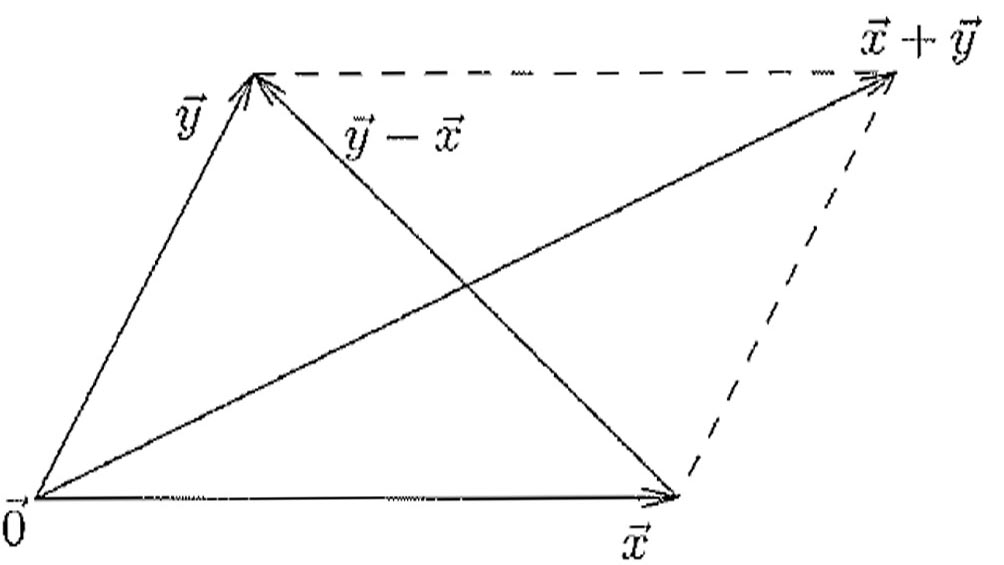
\includegraphics[width=0.5\textwidth]{ParallellogramgelijkheidVlak}
	\caption{Parallellogramgelijkheid in het vlak}
\end{figure}
\end{form}
\item Elke unitaire ruimte is strict genormeerd. Uniciteit is een unitaire ruimte. \\
$\left\{ \begin{array}{ll} ||\vec{x_1}||=||\vec{x_2}||=1\\ \vec{x_1} \neq \vec{x_2} \end{array} \right\} \rightarrow ||x_1 +x_2 || < 2$ \\
$|| x_1+x_2||^2 = 2||x_1||^2+2||x_2||^2-||x_1-x_2||^2 = 4- ||x_1-x_2||^2 \rightarrow ||x_1 +x_2 ||^2 < 4$ \\
Unitair $\rightarrow$ strikt genormeerd
\end{enumerate}
\subsection{Voorbeelden}
Ruimtes die overblijven: \\
\begin{description}
\item [$\mathbb{R}^N\, \mathbb{C}^N$ met $l_2$-norm]
$ (a\vec{x},y)=a(\vec{x},\vec{y}) $ \\
$(x,a\vec{y})=\overline{(a\vec{y},\vec{x})}=\bar{a}\overline{(y,x)}=\bar{a}(x,y)$ \\
$(x,y)=(\sum_{i=1}^n x_i \vec{e_i},\sum_{j=1}^n y_j \vec{e_j})=\sum_{i=1}^n\sum_{j=1}^n  x_i \vec{y_j}(\vec{e_i},\vec{e_j})=X^TG\bar{Y}$

Fundamentele metrische matrix: $G={\begin{vmatrix}\langle e_{1},e_{1}\rangle &\langle e_{1},e_{2}\rangle &\dots &\langle e_{1},e_{n}\rangle \\\langle e_{2},e_{1}\rangle &\langle e_{2},e_{2}\rangle &\dots &\langle e_{2},e_{n}\rangle \\\vdots &\vdots &\ddots &\vdots \\\langle e_{n},e_{1}\rangle &\langle e_{n},e_{2}\rangle &\dots &\langle e_{n},e_{n}\rangle \end{vmatrix}}$ \\

Controleren voor welke p aan de parallellogram gelijkheid voldoet:
2 vectoren (1,1) en (1,-1).
$ ||\vec{x} ||_p = \sqrt[p]{\sum |x_i|^p}$ \\
$ (x,y) = X^TG\bar{Y} $ \\
$\rho(\vec{x},\vec{y}) = \sqrt{(x-y)^TG(x-y)}$ klopt dit wel?  \\ %TODO
\begin{align*}
||x+y ||^2 + ||x-y||^2 &\stackrel{?}{=} 2 ||x||^2+2||y||^2  \\
||(2,0)||^2 + ||(0,2)||^2  &\stackrel{?}{=} 2 ||(1,1)||^2+2||(1,-1)||^2 \\
(\sqrt[p]{2^p+0^p})^2+(\sqrt[p]{0^p+2^p})^2 &\stackrel{?}{=} 2(\sqrt[p]{1^p+1^p})^2+2(\sqrt[p]{1^p+(-1)^p})^2 \\
4 + 4 &\stackrel{?}{=} 2*2^{2/p}+2*2^{2/p} \\
8 &\stackrel{?}{=} 4*2^{2/p} \\
2 &\stackrel{?}{=} 2^{2/p} \rightarrow p=2
\end{align*}
Alleen $p=2$ voldoet aan de parallellogram gelijkheid voldoet, aan al de andere is geen scalair product mee geassocieerd. 

\item [$L_p${[a,b]} met p=2 met $L_2$-norm] 


$(f,g)=\int_a^bw(x)f(x)\bar{g}(x) dx$ \\
$||f||_{L_2} = \sqrt{\int_a^b w(x) f^2(x) dx }$

\item[$l_2 (\mathbb{R}),l_2(\mathbb{C})$ met $l_2$-norm]
\end{description}
Ruimte die afvalt: 
\begin{description}
\item [C{[a,b]}, $max|f(x)|$] 


$f(x)=x$ op [0,1] \\
$g(x)=1$ op [0,1] \\
\begin{align*}
\operatorname{max}^|1+x|^2+\operatorname{max}|x-1|^2 &\neq 2\operatorname{max}|x|^2+2\operatorname{max}|1|^2 \\
2^2+1 &\neq 2+2
\end{align*}

\end{description}

\subsection{Orthogonaliteit}
\begin{enumerate}
\item $ \vec{x} \perp \vec{y}$ als $(\vec{x},\vec{y})=0$
\item $sin \perp cos$ als $(sin,cos)=0$ 
\item $sin \perp 1$
\item $x \perp D$ als $x\perp y$ met $y\in D$
\item Pythagoras als $\vec{x}\perp\vec{y} \rightarrow ||x+y||^2=||x||^2+||y||^2
$ \\
$ (x+y,x+y)=(x,x+y)+(y,(x+y)=(x,x)+(x,y)+(y,x)+(y,y)=(x,x)+(y,y) $
\end{enumerate}
Karakterisatie van beste benadering: Zij u een deelvectorruimte van een unitaire ruimte F en zij $y^* \in y$ zodat $f-y^* \perp y$ dan is $y*$ de beste beatnering voor f in y.
\begin{figure}[h]
	\centering
	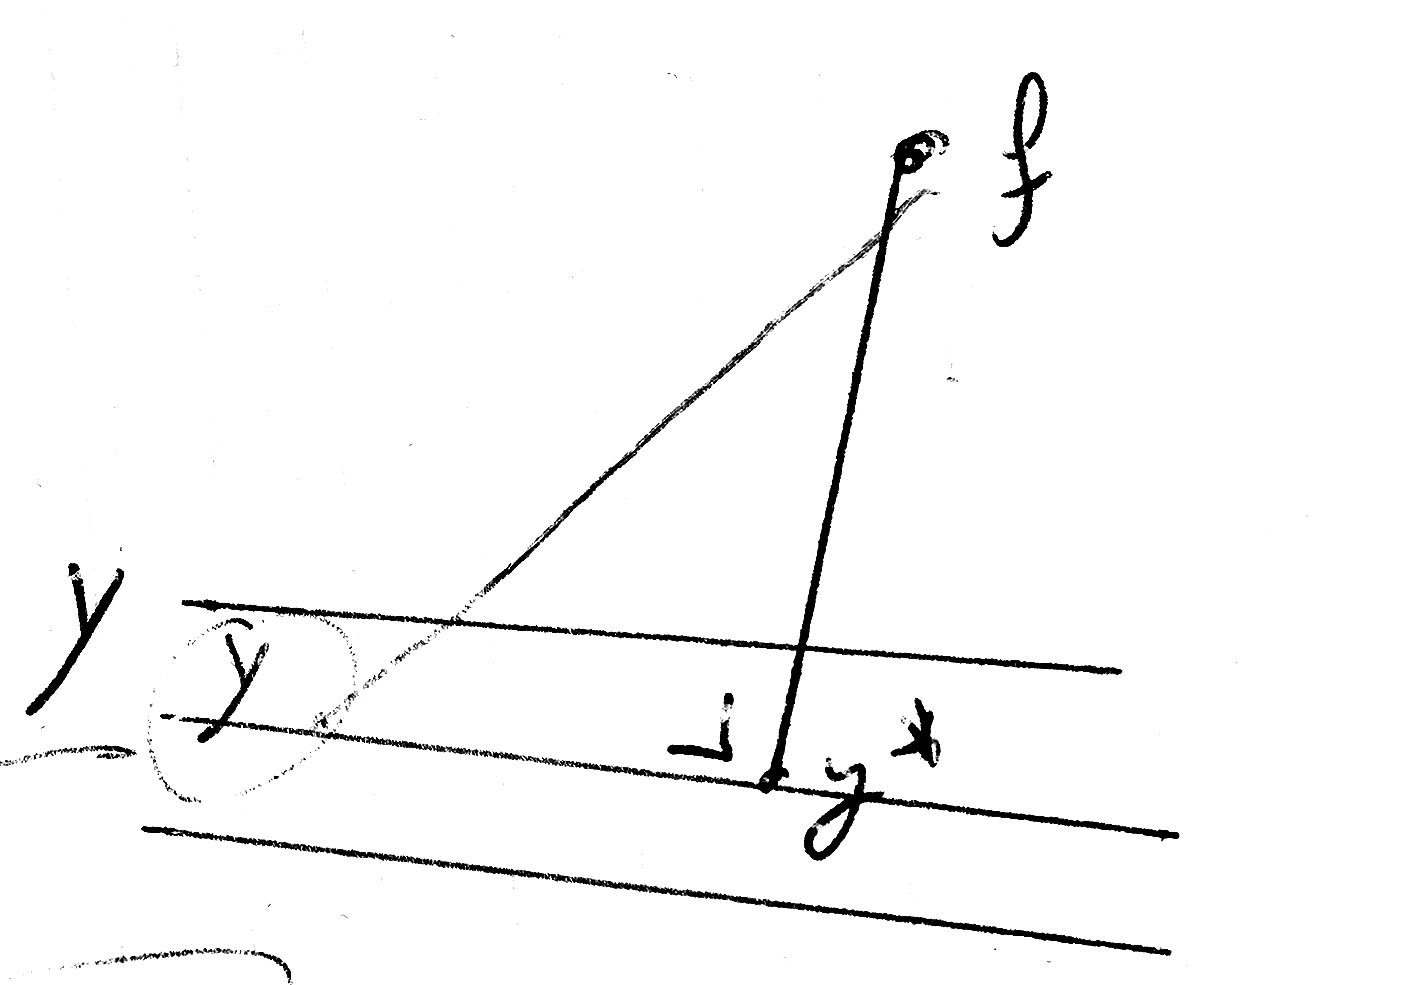
\includegraphics[width=0.5\textwidth]{LoodrechtY}
	\caption{Loodrecht}
\end{figure}
$ ||f-y||^2=||f-y^*||^2+||y-y^*||^2 $ \\
$ ||f-y||^2 \geq ||f-y^*||^2 $ \\
$ \rho(f,y) \geq \rho(f,y^*) $ \\



\section{Euclidische ruimte}
Euclidische ruimte = unitair + eindige dimensionaal, er bestaat een basis , elk element in de ruimte kunnen voorstellen door een aantal getallen (coordinaten).
\begin{figure}[h]
	\centering
	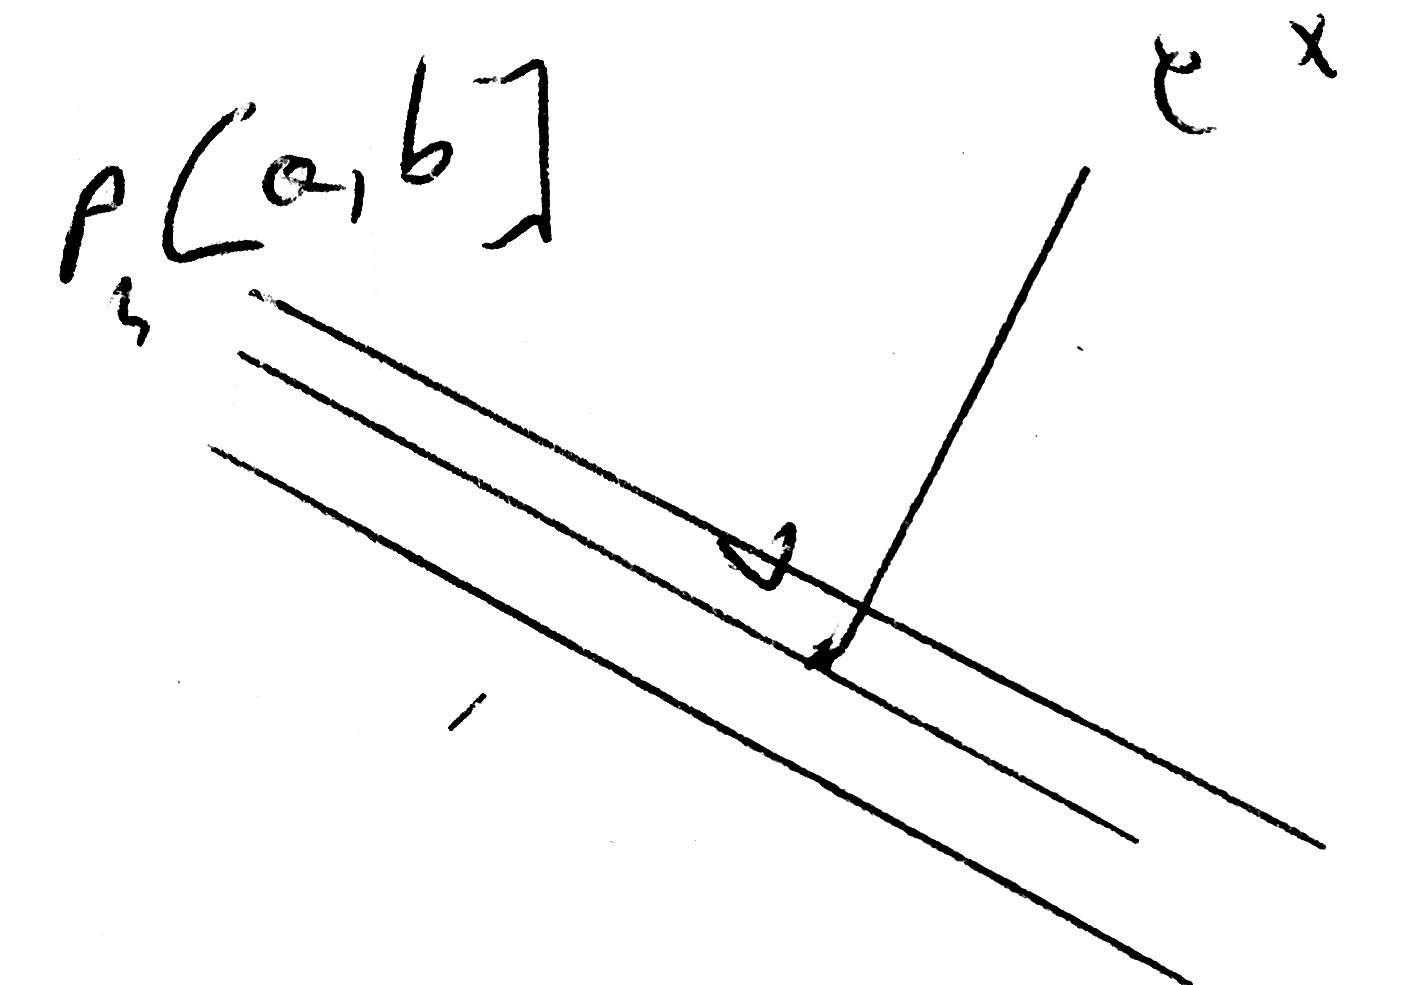
\includegraphics[width=0.5\textwidth]{EuclidischeRuimteLoodrecht2}
	\caption{$e^x$(uit oneindig dimensionale deelruimte) benaderen door een veelterm van graad 4 (5 dimensionale deelruimte)}
\end{figure}
Elke vector kan geschreven worden in de benaderingsruimte plus wat overschiet.
\begin{figure}[h]
	\centering
	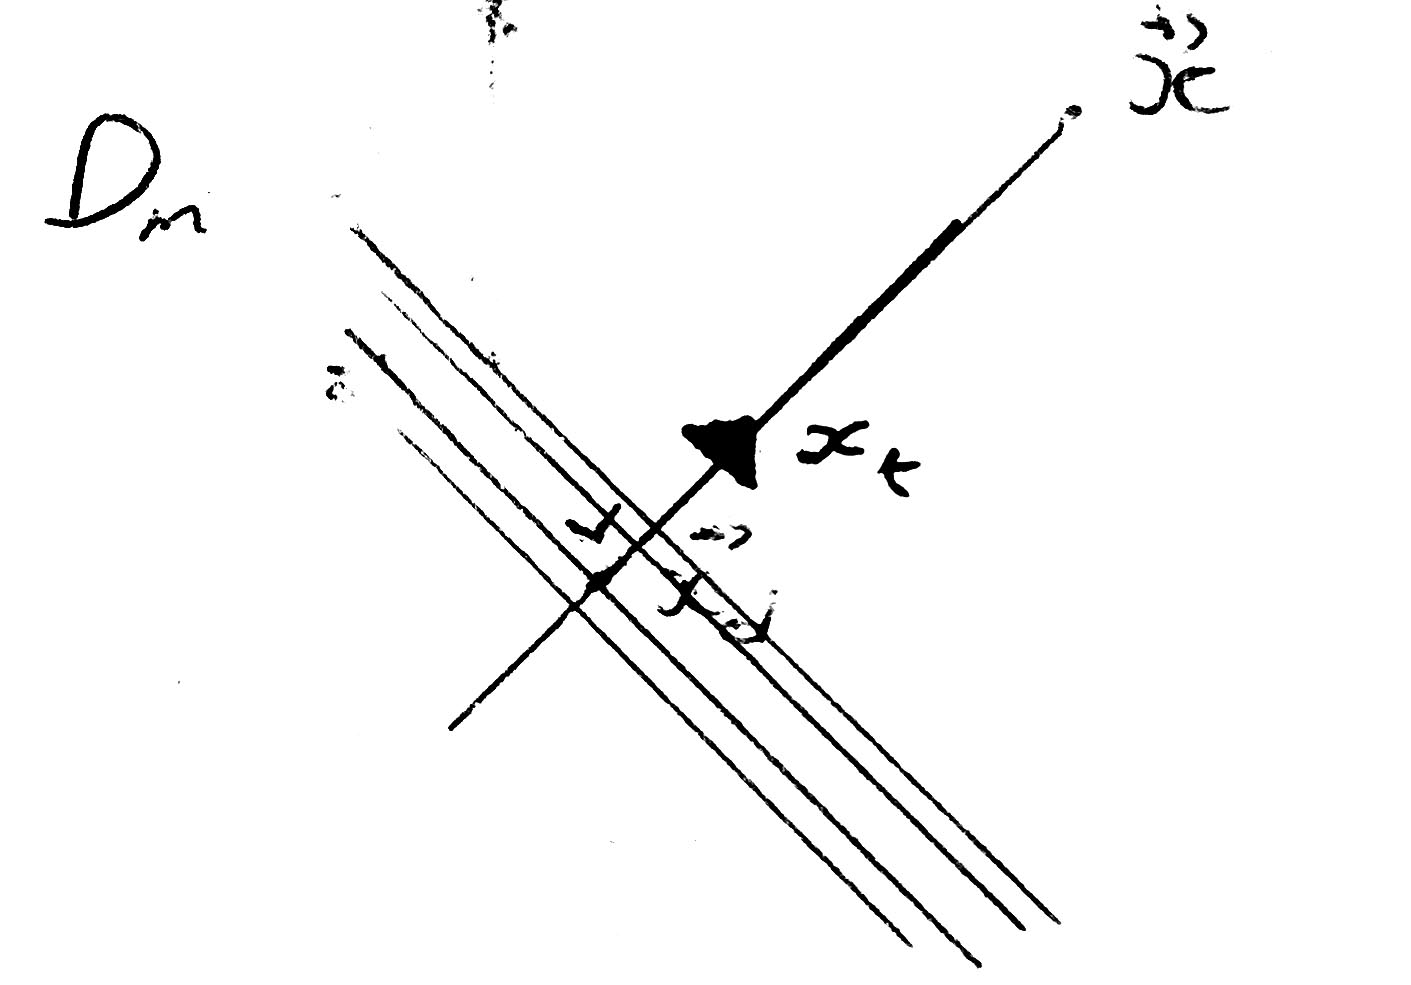
\includegraphics[width=0.5\textwidth]{EuclidischeRuimteLoodrecht}
	\caption{Euclidische ruimte loodrecht}
\end{figure}
$\vec{x}=\vec{x_d}+\vec{x_t}$ met $\vec{x_t}$ residu, benaderingsfout met $\vec{x_d} in D_m$ \\
$\vec{x_t} \perp D_m$ \\
$ \vec{x_d}=\sum_{k=0}^m a_k\vec{e_k} $ stel $\{\vec{e_1},\vec{e_2},\ldots\vec{e_m}\}$ en basis voor $D_m$
(tip: basis kan gaan van k gelijk aan 0 (jaar 2017) of 1 (jaar 2018), is enkel notatie)
Eis:
$\vec{x}-\vec{x_d}\perp \vec{e_i} \,\forall i$ \\
$(\vec{e_1},\vec{x}-\vec{x_d})=0$ $a_1(\vec{e_1},\vec{e_1})+a_2(\vec{e_2},\vec{e_1})+\ldots+a_m(\vec{e_m},\vec{e_1}) = (x,\vec{e_1}) = \sum_{k=1}^m a_k(\vec{e_1},\vec{e_k})=(\vec{e_1},x)$ \\ 
$(\vec{e_2},\vec{x}-\vec{x_d})=0$ $ \sum_{k=1}^m a_k(\vec{e_2},\vec{e_k})=(\vec{e_2},x)$ \\
\vdots \\
$(\vec{e_m},\vec{x}-\vec{x_d})=0$ $ \sum_{k=1}^m a_k(\vec{e_m},\vec{e_k})=(\vec{e_m},x)$ \\
$Ga=b$ (normaalstelsel) met G gramiaanmatrix \\
${\begin{bmatrix}\langle e_{1},e_{1}\rangle &\langle e_{1},e_{2}\rangle &\dots &\langle e_{1},e_{n}\rangle \\\langle e_{2},e_{1}\rangle &\langle e_{2},e_{2}\rangle &\dots &\langle e_{2},e_{n}\rangle \\\vdots &\vdots &\ddots &\vdots \\\langle e_{n},e_{1}\rangle &\langle e_{n},e_{2}\rangle &\dots &\langle e_{n},e_{n}\rangle \end{bmatrix}} * \begin{bmatrix} a_1 \\ a_2 \\ \vdots \\ a_n \end{bmatrix} = \begin{bmatrix} (x,e_1) \\ (x,e_2) \\ \vdots \\ (x,e_n)    \end{bmatrix}  $ \\

Gramiaanmatrix is symmetrisch positief definiet, als re\"el scalair product dat hermetisch positief definiet. \\
Symmetrisch: alleen maar positieve eigenwaarden.
$V^TGV=|| v_1 \vec{x_1} + v_2\vec{x_2} + \ldots +v_m \vec{x_m}||^2$ \\
Positief: $V^TGV > 0$ als $V\neq 0$ \\
Definiet: $V^TGV=0$ als $V=0$ Betekent dat de matrix altijd inverteerbaar is (een reguliere matrix), alle eigenwaarden zijn strict positief. Stelsel altijd een oplossing heeft. Oplossing altijd uniek.
\begin{figure}[h]
	\centering
	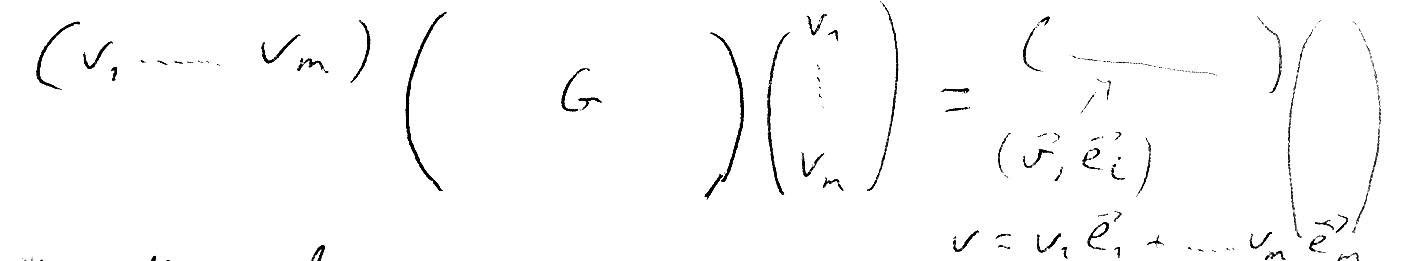
\includegraphics[width=0.5\textwidth]{SPDMatrix}
	\caption{SPD Matrix}
\end{figure}

\subsection{Orthogonale vectoren}
\begin{equation*}
\vec{e_i} \perp \vec{e_j} \, i\neq j
\end{equation*}
\begin{equation*}
a_k = \frac{(\vec{e_k},\vec{x})}{(\vec{e_k},\vec{e_k})} 
\end{equation*}
\begin{equation*}
\vec{x} \approx \vec{x_d} = \sum_{k=1}^m \frac{(\vec{e_k},\vec{x})}{(\vec{e_k},\vec{e_k})}\vec{e_k}
\end{equation*}

Benader $e^x$ in $P_4[-1,1]$
\begin{equation*}
(f,g)=\int_{-1}^1 f.g dx
\end{equation*}
\begin{equation*}
y_4(x)=a_0+a_1x+a_2x^2+a_3x^3+a_4x^4
\end{equation*}
\begin{equation*}
{\begin{bmatrix}\langle 1,1\rangle &\langle x,1 \rangle &\dots &\langle x^4,1\rangle \\\langle 1,x\rangle &\langle x,x \rangle &\dots &\langle x^4,x\rangle \\\vdots &\vdots &\ddots &\vdots \\\langle 1,x^4\rangle &\langle x^2,x^4\rangle &\dots &\langle x^4,x^4 \rangle \end{bmatrix}} * \begin{bmatrix} a_1 \\ a_2 \\ \vdots \\ a_n \end{bmatrix} = \begin{bmatrix} (e^x,1) \\ (e^x,x) \\ \vdots \\ (e^x,x^4)    \end{bmatrix}  
\end{equation*}

\subsection{Gram-Schmidt}
Opstellen van een orthogonale basis. \\
Vertrekt van een schuine basis $\vec{x_1},\vec{x_2},\ldots,\vec{x_m} \rightarrow \vec{y_1},\vec{y_2},\ldots,\vec{y_m}$ orthogonale basis.
\begin{equation*}
\vec{x_1}:\vec{y_1} = \vec{x_1}\lambda_1 \text{ normalisatie}
\end{equation*}
\begin{equation*}
\vec{x_2}:\vec{y_2}=\lambda_2(\vec{x_2}-a_1\vec{y_1}) \text{ met } (\vec{y_2},\vec{y_1})=0
\end{equation*}
\begin{equation*}
a_1 = \frac{(\vec{x_2},\vec{y_1})}{(,\vec{y_1},\vec{y_1})}
\end{equation*}
3 vergelijkingen waar je de 3 getallen kunt halen.
\begin{equation*}
x_i : \vec{y_i} = \lambda (\vec{x_i}-a_1\vec{y_1}\ldots a_{i-1}\vec{y_{i-1}})
\end{equation*}
\begin{equation*}
\rightarrow a_1 = \frac{(\vec{x_i},\vec{y_1})}{(\vec{y_1},\vec{y_1})}
\end{equation*}
\begin{equation*}
\rightarrow a_2 = \frac{(\vec{x_i},\vec{y_2})}{(\vec{y_2},\vec{y_2})}
\end{equation*}
\begin{equation*}
\vec{y_2} \perp \vec{y_1}
\end{equation*}
\begin{equation*}
\vec{y_i} \perp \vec{y_{i-1}}
\end{equation*}
Waar $ || y_2||= ( \vec{y_2},\vec{y_2})=1 $ en $ (\vec{y_i},\vec{y_{i-1}})=0$

\subsubsection{Voorbeeld}
$P_4[-1,1]$ met $(f,q)=\int_{-1}^1 f(x)g(x)dx$ $(L_2)$ \\
$1,x,x^2,x^3,x^4 \rightarrow P_0(x),P_1(x),\ldots,P_4(x)$ \\\\
$1.P_0(x)=\lambda_0.1$ eis $(P_0,P_0)=1$ \\
$\int_{-1}^1\lambda_0^2dx = 1 \rightarrow [\lambda_0^2*x]_{-1}^1 \rightarrow 2\lambda_0^2=1 \rightarrow \lambda_0=\frac{1}{\sqrt{2}}$ \\
$ P_0(x) = \frac{1}{\sqrt{2}}$ \\\\
$x: P_1(x)=\lambda_1(x-a_0P_0(x))$ \\
$a_0=\frac{(x,P_0)}{(P_0,P_0)} = \int_{-1}^1 x \frac{1}{\sqrt{2}} dx = [\frac{x^2}{2 \sqrt{2}}]_{-1}^1=0$\\
$P_1=\lambda_1 x$ \\
Eis $(P_1,P_0)= 0$ \\
$\int \frac{1}{\sqrt{2}}\lambda_1 x dx =0$ \\
Eis$(P_1,P_1)= 1$ \\
$\int \lambda_1x\lambda_1x=1 \rightarrow \int \lambda_1^2 x^2 dx = 1$ \\
$\frac{2\lambda_1^2}{3}=1 \rightarrow \lambda_1 = \sqrt{\frac{3}{2}}$ \\\\
Voor $P_2$ en verder zie boek p34

Voorbeeld: \\
$e^x \approx y_4(x)=a_0+a_1x+\ldots+a_4x^4$ \\
$ = b_0P_0(x)+b_1P_1(x)+\ldots+b_4P_4(x)$\\
\begin{equation*}
b_k = \frac{\int_{-1}^1 e^xP_k(x) dx}{\int_{-1}^1 P_k^2(x) dx}
\end{equation*}
\chapter{Veeltermbenadering (les 3)}
\begin{figure}[h]
	\centering
	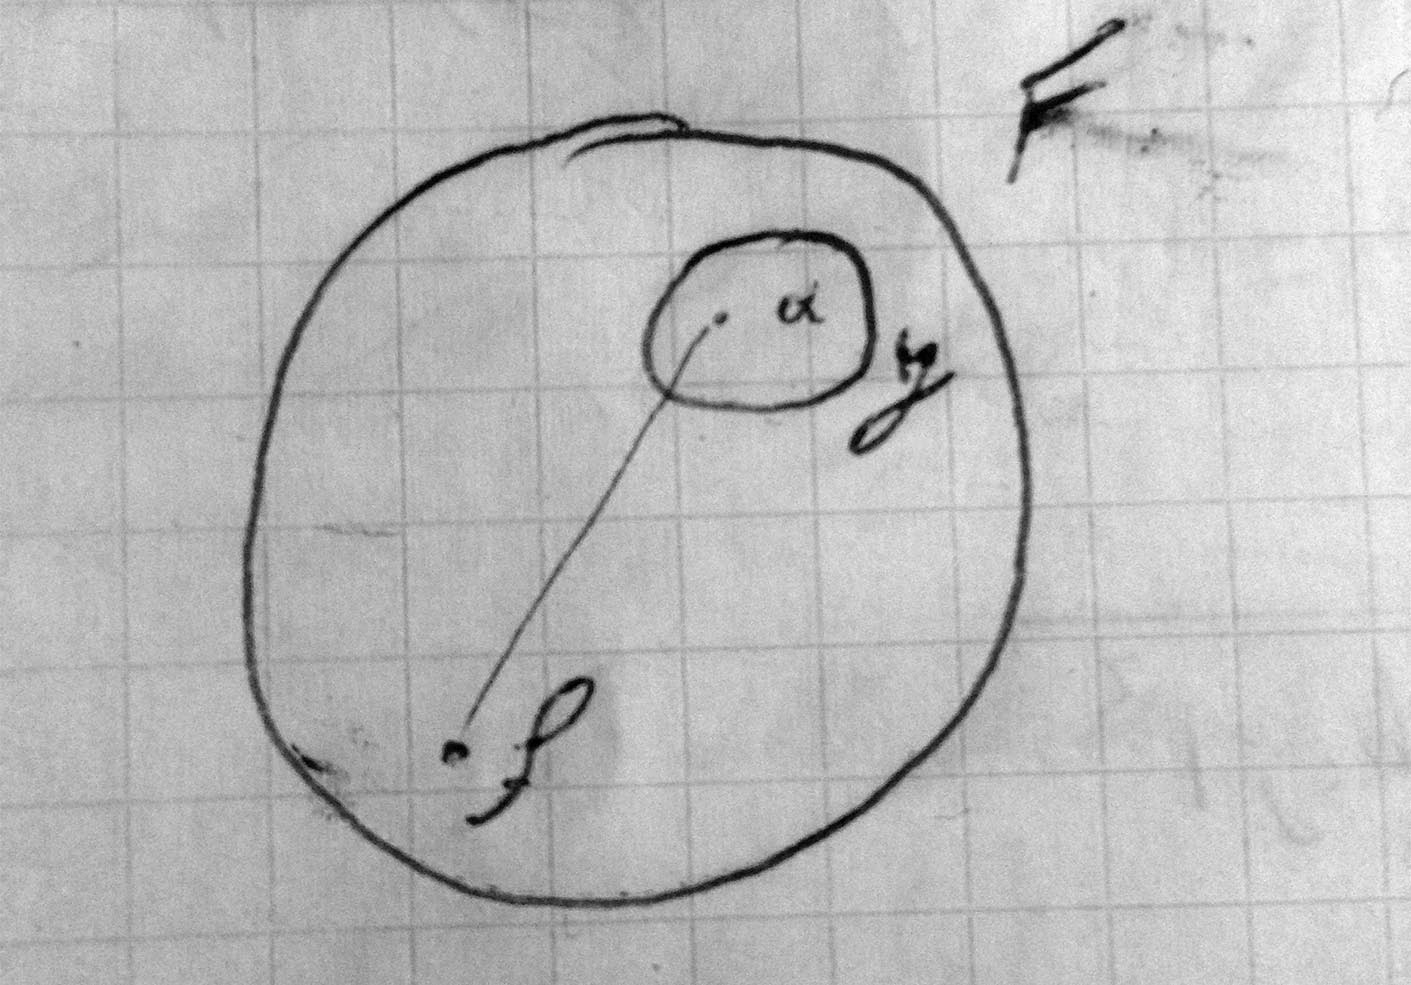
\includegraphics[width=0.5\textwidth]{Benaderingstheorie}
	\caption{Benaderingstheorie}
\end{figure}
\section{Continue benadering}
$F=C[a,b]$ of $F=L_2[a,b]$ \\
$Y \subset F$ \\
$y=P_n[a,b]$ (veelterm van graad n)\\
$(f,g)=\int_a^b w(x)f(x)g(x)dx$ , $w(x) >0 a.e.$ \\
$w(x)$ mag niet te moeilijk zijn $\int_a^b w(x) x^k dx < \infty$ 
\section{Discrete benadering}
F=$\mathbb{R}^N$, $\mathbb{C}^N$, $l_2$ \\
$y= P_n[a,b]$ \\
$(f,g)=\sum_{i=1}^N w_i f_i g_i$ $l_2$-scalair product. \\
$Y \subset F$ Een veelterm is een continu iets, niet echt een deelverzameling van $\mathbb{R}^N$ maar dat is oplosbaar. Je kunt die $mathbb{R}^N$, zijn N getallen, je kan dit interpreteren, door elke vector van N getallen gaat precies 1 veelterm van graad N-1. Dit is isomorf aan de hogere dimensionale veelterm ruimte. \\

\section{Klassieke basis}
$f \approx y_n(x)= \sum_{k=0}^n a_k \phi^k$ \\
$w(x) \equiv 1$ \\
$[a,b]=[0,1]$ 
\begin{enumerate}
\item Klassieke keuze $\phi_k(x)=x^k$ (monomiale basis) \\
${\begin{bmatrix}\langle 1,1\rangle &\langle x,1 \rangle &\dots &\langle x^4,1\rangle \\\langle 1,x\rangle &\langle x,x \rangle &\dots &\langle x^4,x\rangle \\\vdots &\vdots &\ddots &\vdots \\\langle 1,x^4\rangle &\langle x^2,x^4\rangle &\dots &\langle x^4,x^4 \rangle \end{bmatrix}} * \begin{bmatrix} a_1 \\ a_2 \\ \vdots \\ a_n \end{bmatrix} = \begin{bmatrix} (e^x,1) \\ (e^x,x) \\ \vdots \\ (e^x,x^4)    \end{bmatrix}  $

Continu: $(f,g)=\int{a=0}^{b=1} f(x)g(x) dx \rightarrow (x^i,x^j)= \int{a=0}^{b=1} x^{i+j}dx = \frac{1}{i+j+1}$ \\
Discreet: $(f,g)=\sum_{k=1}^N f_i g_i \rightarrow (x^i,x^j)= N \sum_{k=1}^N w_k x_k^{i+j}\frac{1}{N} \approx N \int_0^1 x^{i+j} dx$ \\



\begin{figure}[h]
	\centering
	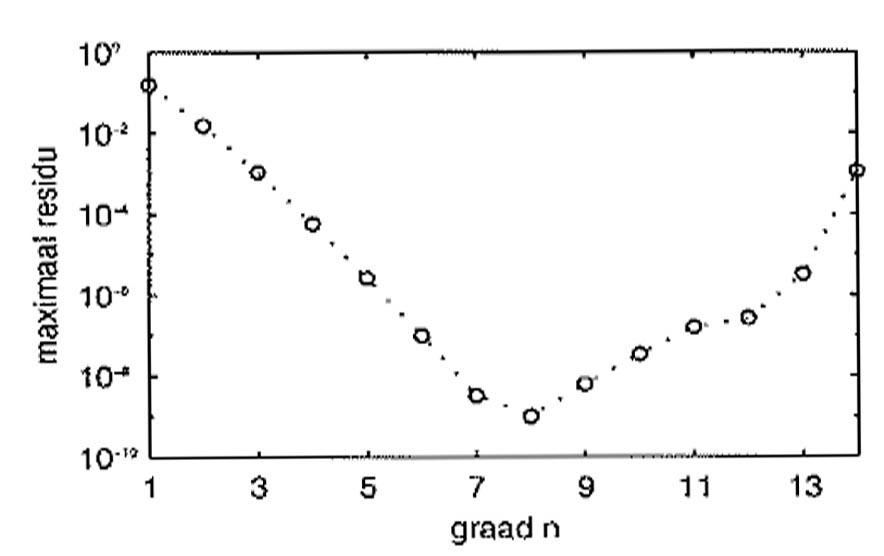
\includegraphics[width=0.5\textwidth]{MaxResiduMonomialeBasis}
	\caption{Max residu met een monomiale basis}
\end{figure}
Ergens wordt de afwijking tussen benadering en de te benaderen functie ($e^x$) maximaal, deze afwijking is weergegeven per graad. Er is een merkwaardig effect dat de fout plots gaat stijgen, de benadering wordt niet beter zelf slechter, wat eigenlijk niet zou mogen zijn, want de benaderingsruimte als je de graad ophoogt dan wordt de benderingsruimte  maar groter en groter en zou de benadering beter moeten worden. Het stijgen dit komt door voortplanting van afrondingsfouten.
$Ga=b$ hieruit a zoeken, dan doe je dat met een numerieke methode. De mate van toename komt overeen met de conditie van de matrix. $K(G) = ||G||||G^{-1}||$. 
Voorbeeld: $n=4 \, K(G) \sim 47000=1$ Verliezen 5 aantal decimale cijfers \\ $n=10 K(G) \sim 10^{13}$ \\

Moest je de inverse van $G$ berekenen (wat normaal niet expliciet wordt gedaan), kan je zien dat er afwisselend grote negatief en positieve getallen. Als je grote getallen met elkaar combineert en je komt iets klein uit, dan verliest men nauwkeurigheid.
\item Orthogonale basis \\
$y_n(x)= \sum_{k=0}^n a_k \phi^k$ \\
$a_k = \frac{(e^x,P_k)}{(P_k,P_k)}$ \\

\begin{figure}[h]
	\centering
	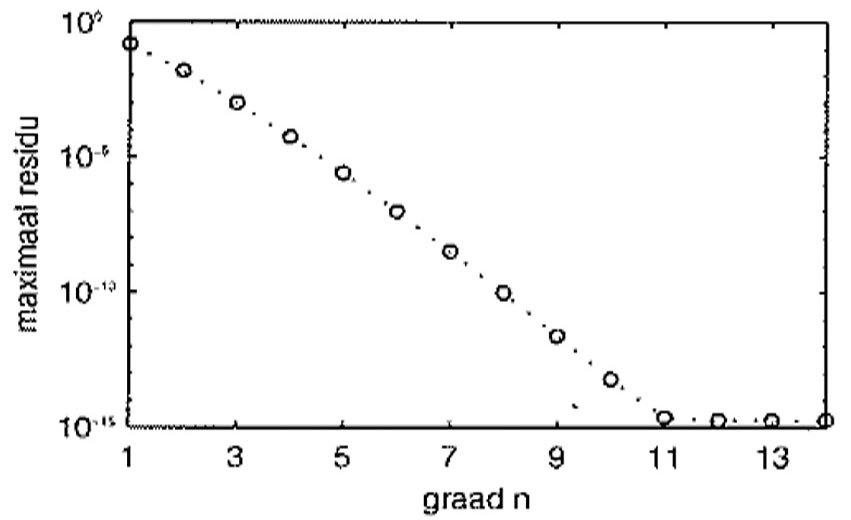
\includegraphics[width=0.5\textwidth]{MaxResiduOrthogonaleBasis}
	\caption{Max residu met een orthogonale MonomialeBasis}
\end{figure}


Eigenschappen 
\begin{enumerate}
\item 
$\phi_0(x),\phi_1(x),\phi_2(x),\ldots,\phi_k(x)$
$\phi_k \perp \phi_{k-1} \in \phi_{k-1}[a,b]$ of $ \phi_k \perp \phi_{k-1},\phi_{k-2},\ldots \phi_0$ Alsook tot alle lineaire combinaties van $\phi$ $\rightarrow \phi_k \perp \phi_{k_1}[a,b]$

Er is een gemakkelijkere manier om $\phi_k$ op te stellen dan de gramm-schmidt methode. Er bestaat een recursiebetrekking, deze zegt dat $\phi_k$ kan berekent worden aan de hand van zijn 2 voorgangers  $\phi_{k-1}$ en $\phi_{k-2}$. Deze recursie moet natuurlijk opgestart worden: $\phi_0(x)=\lambda_0$ en  $\phi_1(x)=\lambda_1(x-\alpha_1)\phi_0$ met $\alpha_1 = \frac{(x,1)}{(1,1)}$. \\
$\{1,x\} \rightarrow \{\phi_0,\phi_1\}$ \\
$x \rightarrow \phi_1 = \lambda_1 \frac{( x- \phi_0)}{( \phi_0- \phi_0)}= \lambda_1 (x-\frac{( x- 1)}{( 1-1)})$ \\ Om formule mooi te laten overeenkomen met de recursiebetrekking voegt men nog $\phi_0$ toe.
$x \rightarrow \phi_1 = \lambda_1 \frac{( x- \phi_0)}{( \phi_0- \phi_0)}\phi_0 = \lambda_1 (x-\frac{( x- 1)}{( 1-1)})\phi_0 $ \\

Bewijs recursiebetrekking:
$x \phi_{k-1}= b_0\phi_0 + b_1 \phi_1 + \ldots + b_k \phi_k $ \\
$b_0 = \frac{(x\phi_{k-1},\phi_0)}{(\phi_0,\phi_0)} = \frac{(\phi_{k-1},x\phi_0)}{(\phi_0,\phi_0)}=0$ \\
Hoge graads veelterm $\phi_{k-1}$ staat loodrecht op alles lager dan $\phi_{k-1}$ dus ook op $\phi_0 \rightarrow 0$ \\
$b_1 = \frac{(x\phi_{k-1},\phi_1)}{(\phi_1,\phi_1)} = \frac{(\phi_{k-1},x\phi_1)}{(\phi_1,\phi_1)}=0$ \\
$\vdots$\\
$b_{k-3} = \frac{(x\phi_{k-1},\phi_{k-3})}{(\phi_{k-3},\phi_{k-3})} = \frac{(\phi_{k-1},x\phi_{k-3})}{(\phi_{k-3},\phi_{k-3})}=0$ \\
$b_{k-2} = \frac{(x\phi_{k-1},\phi_{k-2})}{(\phi_{k-2},\phi_{k-2})} = \frac{(\phi_{k-1},x\phi_{k-2})}{(\phi_{k-2},\phi_{k-2})}$ \\
$b_{k-1} = \frac{(x\phi_{k-1},\phi_{k-1})}{(\phi_{k-1},\phi_{k-1})} = \frac{(\phi_{k-1},x\phi_{k-1})}{(\phi_{k-1},\phi_{k-1})}$ \\
$b_{k} = \frac{(x\phi_{k-1},\phi_{k})}{(\phi_{k-3},\phi_{k})} = \frac{(\phi_{k-1},x\phi_{k})}{(\phi_{k},\phi_{k})}$ \\
$x \phi_{k-1}= b_{k-2}\phi_{k-2} + b_{k-1}\phi_{k-1} +b_{k}\phi_{k} $ \\

$\phi_k(x)= \frac{1}{b_k}(x-b_{k-1})\phi_{k-1}-\frac{b_{k-2}}{b_k}\phi_{k-2}$ \\

$\phi_k(x) = \lambda_k(x-\alpha_k)(\phi_{k-1}(x)-\beta_k\alpha_{k-2}(x)$ \\
$\lambda_k= \frac{1}{b_k}$ \\
$\alpha_k = b_{k-1} = \frac{(x\phi_{k-1},\phi_{k-1})}{(\phi_{k-1},\phi_{k-1})}$ \\
$\beta_k = \frac{b_{k-2}}{b_k} = \lambda_k b_{k-2} = \lambda_k \frac{(x\phi_{k-1},\phi_{k-2})}{(\phi_{k-2},\phi_{k-2})}$ \\
$\lambda$ kan niet  uitgerekend worden, in de formule gebruik je al $\phi_k$ , die $\lambda$ is een normalisatie constante, die zal de lengte van de vector bepalen, in een orthogonale basis doet het er niet toe welke lengte je geeft aan de vectoren, meestal zetten $\lambda=1$, dan hebben we geen extra rekenwerk maar zijn niet alle vectoren even lang. \\
Voorbeeld: \\
$w(x) \equiv 1$ \\
$[a,b]=[-1,1]$, Legendre-veeltermeen $P_k(x)$ \\
$P_k(x)= \lambda_k (x-\alpha_k)P_{k-1}(x)-\beta_kP_{k-2}(x)$ \\

\item $\phi_k(x)$ heeft juist k enkelvoudig nulpunten in het open interval (a,b). Betekent buiten dit interval gaat men naar + of - oneindig. \\
Bewijs stel $m<k$ enkelvoudige nulpunten (tekenwisselingen) in het open interval (a,b) (bewijs uit het ongerijmde) 
\begin{figure}[h]
	\centering
	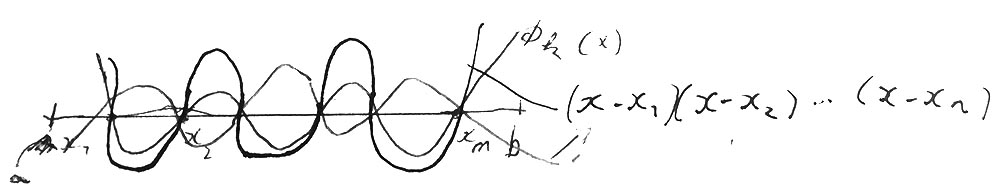
\includegraphics[width=0.5\textwidth]{ProveKEnkelvoudigeNulpunten}
	\caption{Bewijs k enkelvoudige nulpunten}
\end{figure}

$\Psi_k(x)=\phi_k(x)(x-x_1)\ldots(x-x_m)$ \\
Elke tekenverandering van $\phi_k$ wordt teniet gedaan door een tekenverandering van de gewone functie. Dit betekent dat het product van deze altijd hetzelfde teken moet hebben. $\Psi_k$ is overal positief of negatief dus $\int_a^b w(x) \Psi_k(x) dx \neq 0$. Is in tegenspraak met $\phi_k(x) \perp \Psi(x)$ .

\end{enumerate}
\end{enumerate}
%Subdivisie
%Periodieke spline 
%Leg het belang van orthogonale veeltermen uit. Hoe worden deze opgesteld en genormaliseerd? Bewijs de recursiebetrekking voor orthogonale veeltermen. Illustreer deze betrekking door de eerste 3 Legendre veeltermen te berekenen. Waarvoor zijn de nulpunten van deze veeltermen nuttig?

%Bézier: Eigenschappen verklaren aan de hand van Bernsteinveeltermen. Curve grafisch voorstellen. Wat is het nut van Béziercurven? (In de praktijk enkel tekenen van fonts) Bewijs dat de rationale een kegelsnede exact kan voorstellen. Bijvragen: Wat is nu het feitelijke belang van een affiene combinatie? Welke punten gebruik je voor het evalueren van de curve? Wat is het verschil tussen Metafont en Postscript? Toon aan welke kegelsnede je wanneer krijgt? 

%Bewijs het Danielson-Lanczos splitsingsalgoritme. Leg uit hoe men met dit algoritme komt tot het FFT algoritme. Gegeven een FFT/IFFT algoritme van complexe rijen, leid een algoritme af om twee getallen van 10000 cijfers met elkaar te vermenigvuldigen.

%Wat zijn Affiene en Convexe combinaties? Waarom zijn ze zo intressant voor het gebruik in grafische modelering? Verklaar met veelterminterpolatiecurven, alsook beziercurven. Waarom zijn rationale veeltermcuvern zo intressant? Bewijs dat met 2e graads rationale curven kegelsnedes kunnen voorgesteld worden.  Waarom zijn NURBS zo intressant? 
%stel de onderstaande curven grafisch voor. Maak voor elk puntje een duidelijke tekening. Maak geen berekeningen. 5 controlepunten van de beziercurve : (0,0), (0,1), (1,1), (1,0), (2,1). - teken het gebied waarin de bezier-curve kan liggen. Op welke eigenschap steun je hiervoor? In welk gebied kunnen spline-curven liggen? - Duidt aan op de figuur waar het punt met t = 0.25 ligt + geef de afleiding van het algoritme dat je hiervoor gebruikt. - voeg nu een controlepunt toe zonder dat de vorm van de curve verandert. Welke eigenschap gebruik je hiervoor? - Teken de controleveelhoek voor t = [0, 0.5]

%Vergelijk het gebruik van interpolerende veeltermen, Bernstein-veeltermen, spline-functies en NURBS voor het modelleren van curven. Geef telkens de definitie, de belangrijkste eigenschappen en het overzicht van de voor- en nadelen. Bewijs dat een rationale Bézier-curve van graad 2 overeenstemt met een boog van een kegelsnede. 

%Het FFT-algoritme kan gebruikt worden voor het berekenen van de DFT van een complexe rij. Leg uit hoe je dit algoritme moet aanpassen om op een efficiënte wijze de DFT en de DCT te berekenen van een reële rij. Bewijs de stellingen waarop die aanpassingen gebaseerd zijn! Leg uit hoe je de DFT en de DCT van een digitaal beeld kunt berekenen. Wat is de rekencomplexiteit als je de FFT gebruikt? Waarom verkiest men doorgaans de DCT?

%Toon aan hoe de vorm van een Bézier-curve volgt uit de eigenschappen van de Bernsteinveeltermen. Hoe tekent men een Bézier-curve? Illustreer met een duidelijke tekening. Bewijs dat een rationale Bézier-curve van graad 2 overeenstemt met een boog van een kegelsnede. 


%Geef gedetailleerd hoe B-splines gebruikt kunnen worden om een kleinste kwadraten benadering op te stellen. Hoe ziet de structuur van de matrix eruit? Wat verandert er als we willen benaderen in meerdere veranderlijken? 
%Bespreek gedetailleerd de methode voor veeltermvermenigvuldiging. Wanneer we 2 getallen met elk 1000000 (10^6) cijfers willen vermenigvuldigen in hoge nauwkeurigheid en een FFT algoritme ter beschikking hebben, hoe zouden we dan concreet te werk gaan? Leg gedetailleerd uit, bespreek ook per stap de complexiteit van de berekeningen. Hoe werkt dit voor reële getallen? Deling?
%Definieer Splines en B-Splines, bewijs recursiebetrekking voor B-splines en gebruik recursiebetrekking om positiviteit te bewijzen. Bespreek splines met meervoudige knooppunten. 

%Nulpunten orthogonale veeltermen: Hoe vind je ze, hoeveel zijn er (+bewijs), waarom zijn ze goed als interpolatiepunten.
%leg het belang van orthogonale veeltermen uit. Bewijs de drietermrecursiebetrekking en stel de legendre veeltermen tot en met graad 3 op. Wat is het nut van de nulpunten te kennen en hoe bepaal je ze.

%Geef de definities van affiene en convexe combinaties. Wat is het belang binnen CAGD, gebruik veeltermen en bezier als vb. Waarom gebruikt men rationale curven, welke types zijn er? Bewijs dat rationale bezier, van graad 2 de boog van een kegelsnede is ... 

%Geef de formules voor DCT/IDCT. Hoe leid je deze af uit de orthogonalisatie eigenschappen van de cosinusfunctie? (HB p.91) Hoe reken je dit uit met FFT? (Bewijs) Waarom wordt bij beeldcompressie eerder DCT gebruikt dan DFT? Leg beknopt het JPEG algoritme uit. Bijvragen: Waarvoor staat JPEG? Welke compressiemethode gebruikt men tegenwoordig nog?

%Wat is een kubische spline-functie? Hoe groot is de dimensie van de spline ruimte? Geef én teken een basis van afgeknotte machtsfuncties en een basis van B-splines. Bewijs dat B-splines een compacte drager voortbrengen (dat de basis beperkt is over een interval; m.a.w. Bewijs Stelling 2 HB p.118). Leg gedetailleerd uit hoe je een experimenteel bepaalde curve zou benaderen met een basis van B-splines. (Welk benaderingscriterium gebruik je? Hoe ziet het bekomen stelsel er uit? Hoe zou je dit stelsel oplossen?) Bijvragen: Oplossen met normaalstelsel: Hoe ziet de gramiaan eruit? (bandstructuur); Als je stelsel oplost met QR-factorisatie: Hoe zou je deze QR-factorisatie uitvoeren? Wat is er voordelig aan Givens rotatie? (HB p.138) 

%geef de definitie van splinefunctie. Leid de dimensie van de splineruimte af. Hoe definiëren we splinefuncties met samenvallende knooppunten? geef en verklaar de continuïteitseigenschappen. teken op de figuur (gegeven, met knooppunten) de eerste, tweede en derde basisfunctie en verklaar de discontinuiteit. 

%Leid Danielson-Lanczos af. Wat is het nut hiervan voor het berekenen van een DFT. DFT van een Reele rij. Vermenigvuldigen van grote getallen.

%5 punten gegeven, elk vraag over punten grafisch weergeven: Waarbinnen ligt de Bezier curve? Waar is het punt dat overeenkomt met t=0.25? Bewijs de gebruikte eigenschap. Hoe stel je dezelfde curve voor met 6 punten en welke eigenschap heb je hiervoor nodig? Wat zijn de 5 punten die overeenkomen met t = [0.5...1]? Wat is hier een belangrijke toepassing van? 
\chapter{xx}

\section{x}
\chapter{xx}

\section{x}
\chapter{xx}

\section{x}
\chapter{Oefenzittingen}
\section{Oefenzitting 1 - Benaderingstheorie}
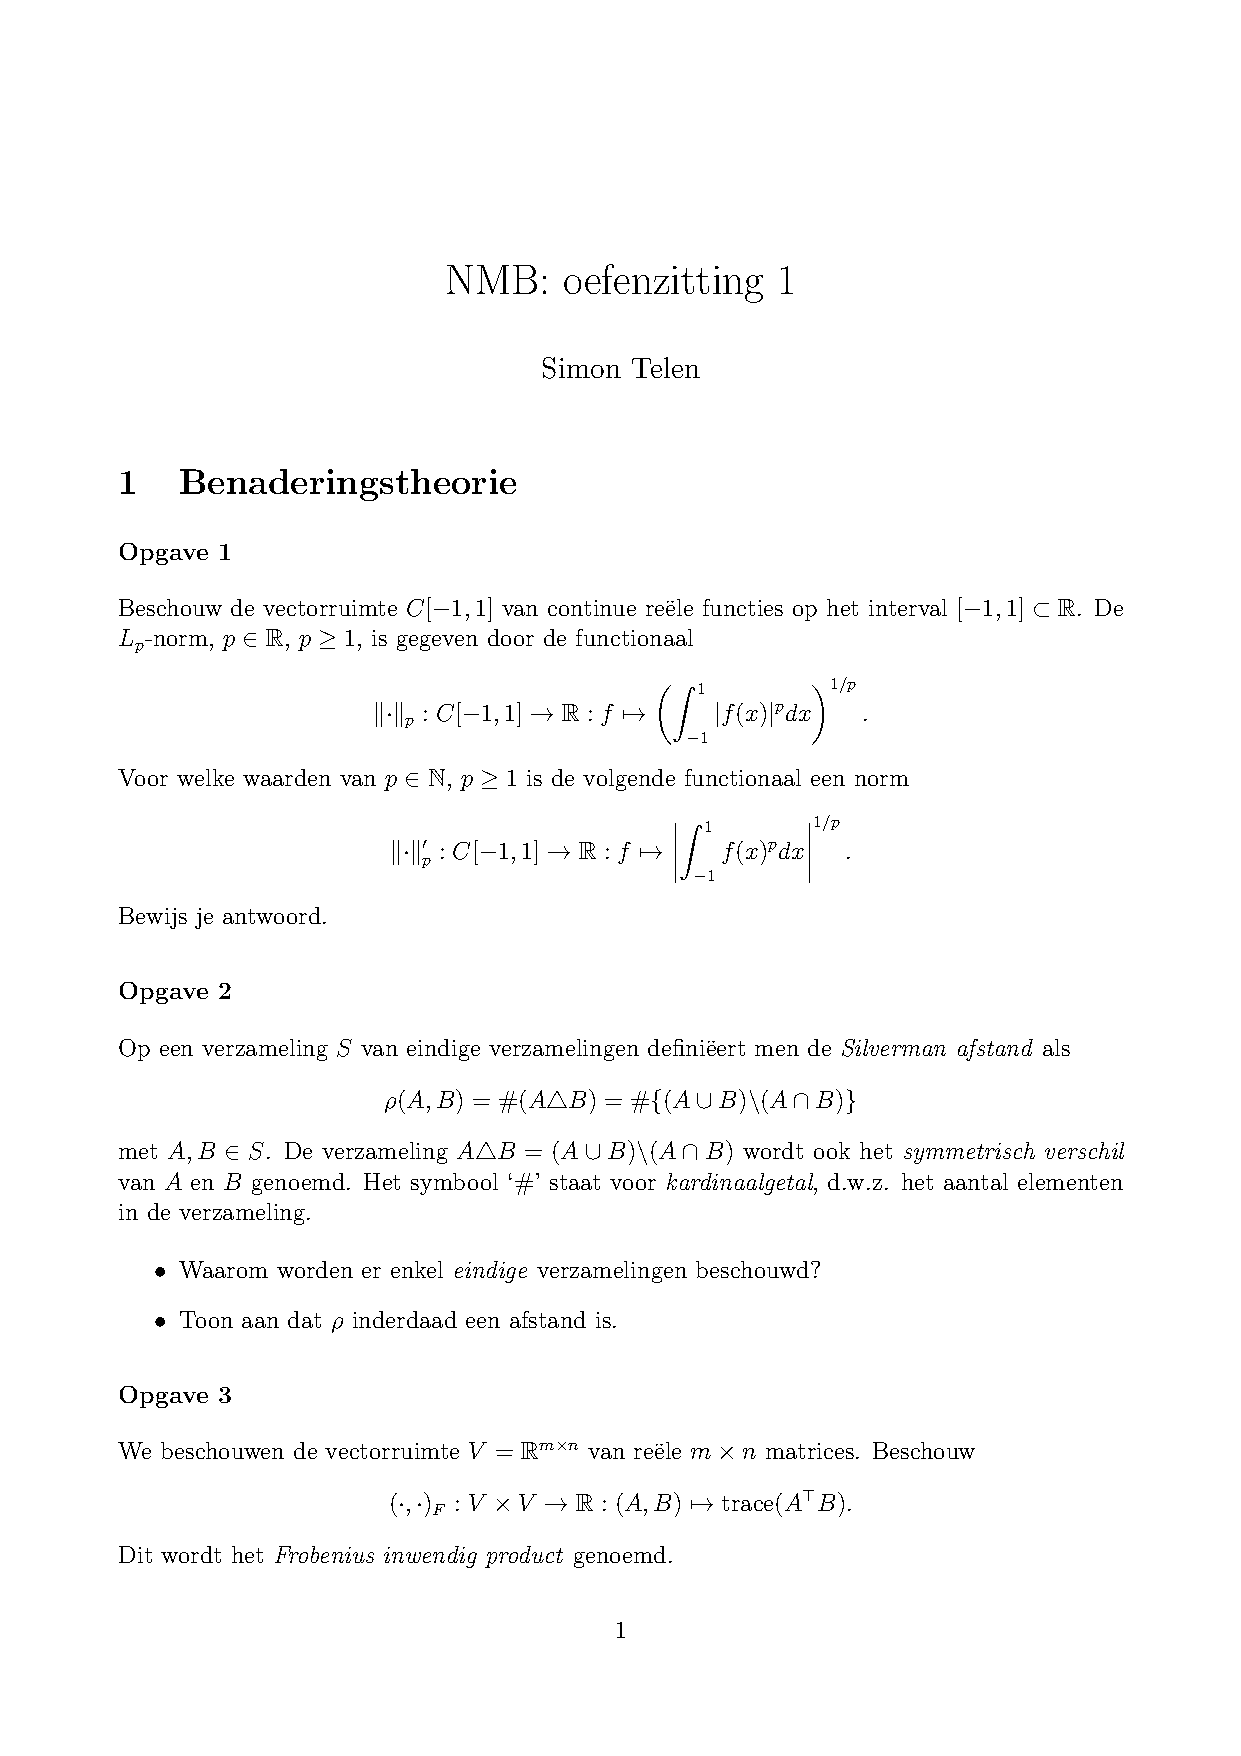
\includepdf[pages=-,frame,scale=0.7,pagecommand={}]{exercise/1_opgave1.pdf}
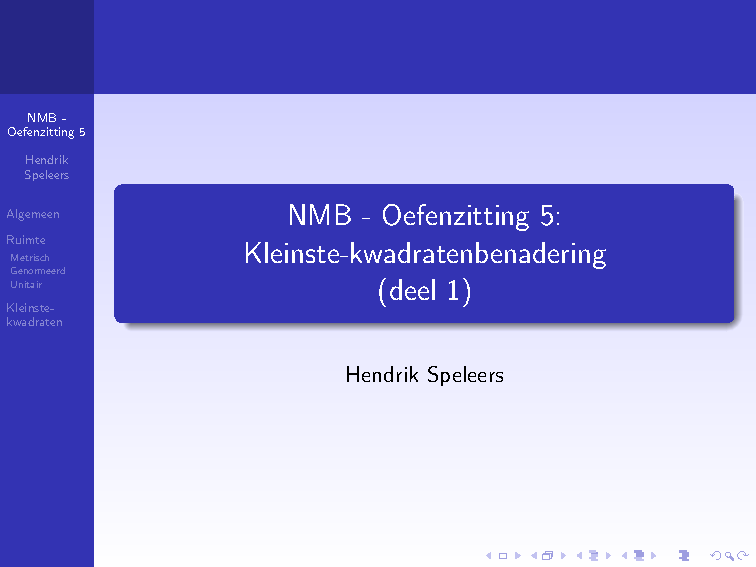
\includepdf[pages=-,frame,scale=0.7,pagecommand={},nup=2x3]{exercise/1_slides5.pdf}
\subsection{Oplossingen}
%\include{exercise/Session2}
%\include{exercise/Session3}
%\include{exercise/Session4}
%\include{exercise/Session5}
%\include{exercise/Session6}
%\include{exercise/Session7}
%\include{exercise/Session8}
% Appendix
\appendix

% References
\bibliographystyle{plain}
\bibliography{bibliography}
\nocite{*}

\end{document}

